\section{Group -- Simulation Parameters}\label{group-simulation-parameters}

This group of objects influences the simulation in various ways.

\subsection{Version}\label{version}

\subsubsection{Inputs}\label{inputs-044}

\paragraph{Field: Version Identifier}\label{field-version-identifier}

The Version object allows you to enter the proper version that your IDF was created for. This is checked against the current version of EnergyPlus and a Severe error issued (non-terminating) if it does not match the current version string. Note that versions are often significant and there is no guarantee that the older file will run in the newer versions of the program. See IDF Version Updater (Auxiliary Programs Document) for methods of changing the older files to newer versions.

\subsection{Timestep}\label{timestep}

\subsubsection{Inputs}\label{inputs-1-041}

\paragraph{Field: Number of Timesteps per Hour}\label{field-number-of-timesteps-per-hour}

The Timestep object specifies the ``basic'' timestep for the simulation. The value entered here is usually known as the Zone Timestep. This is used in the Zone Heat Balance Model calculation as the driving timestep for heat transfer and load calculations. The value entered here is the number of timesteps to use within an hour. Longer length timesteps have lower values for Number of Timesteps per Hour. For example a value of 6 entered here directs the program to use a zone timestep of 10 minutes and a value of 60 means a 1 minute timestep. The user's choice for Number of Timesteps per Hour must be evenly divisible into 60; the allowable choices are 1, 2, 3, 4, 5, 6, 10, 12, 15, 20, 30, and 60.

The choice made for this field has important implications for modeling accuracy and the overall time it takes to run a simulation. Here are some considerations when choosing a value:

\begin{itemize}
    \item
    The solution technique used in EnergyPlus has been designed to be stable with zone timesteps of up to sixty minutes (Number Timesteps in Hour = 1). However, 60 minutes is considered a ``long'' timestep and it should only be used in rare occasions where there is no HVAC system, accuracy is not a concern, and short run times are critical. Such long timesteps are not recommended to use because simulation results are more accurate for shorter timesteps, of say 10 minutes or less (Number of Timesteps per Hour of 6 or more). Shorter zone timesteps improve the numerical solution of the Zone Heat Balance Model because they improve how models for surface temperature and zone air temperature are coupled together. Longer timesteps introduce more lag and lead to more a dampened dynamic response.
    \item
    Simulation run time increases with shorter timesteps or larger values for Number of Timesteps per Hour. The effect varies with the nature of the model. The user can test out different values on their particular model to understand the implications for his or her particular case. Sometimes large models with multizone HVAC and Plant systems execute nearly as fast with 15 minute timesteps as with 60 minute timesteps because fewer iterations are required in the system modeling since the prior timestep's results are close to the final outcome of next timestep.
    \item
    The weather data files usually have 60-minute (or hourly) data. However, it does not follow that this should be used as the basis for choosing the zone timestep because:
    \item
    EnergyPlus carefully interpolates the weather data between data points for use at shorter timesteps. This is discussed in a later section: Weather Data Hourly Interpolation
    \item
    Many aspects of a model have time scales that differ from the that of the weather data. A goal of the modeling is to predict how the building will respond to the weather. However, the building's response is not \emph{governed} by the time scale that the weather data are available at, but rather the time scales of the dynamic performance of the thermal envelope as well as things like schedules for internal gains, thermostats, and equipment availability.
    \item
    If the model will include calculating the cost of electricity, then the user should be aware that many electric utility tariffs base charges on demand windows of a specified length of time. If the choice of Number of Timesteps per Hour is not consistent with the demand window, then unexpected results may be obtained. For reasonable prediction of the maximum rates for electricity use for in calculating demand charges, the length of the zone timestep needs to be consistent with the tariff's demand window. The following table lists what values are consistent with various demand windows.
\end{itemize}

\begin{longtable}[c]{@{}ll@{}}
    \toprule
    Demand Window & Applicable Number of Timesteps per Hour \tabularnewline
    \midrule
    \endfirsthead

    \toprule
    Demand Window & Applicable Number of Timesteps per Hour \tabularnewline
    \midrule
    \endhead

    QuarterHour & 4, 12, 20, or 60 \tabularnewline
    HalfHour & 2, 4, 6, 10, 12, 20, 30, or 60 \tabularnewline
    FullHour, Day, Week & Any \tabularnewline
    \bottomrule
\end{longtable}

There is also second type of timestep inside EnergyPlus that is known as the System Timestep. This is a variable-length timestep that governs the driving timestep for HVAC and Plant system modeling. The user cannot directly control the system timestep (except by use of the \hyperref[convergencelimits]{ConvergenceLimits} object). When the HVAC portion of the simulation begins its solution for the current zone timestep, it uses the zone timestep as its maximum length but then can reduce the timestep, as necessary, to improve the solution. The technical details of the approach are explained in the Engineering Documentation under ``Integrated Solution Manager''.

Users can see the system timestep used if they select the ``detailed'' frequency option on an HVAC output variable (e.g. Zone Air Temperature). To contrast, the ``Zone'' variables will only be reported on the zone timestep (e.g. Zone Mean Air Temperature).

And, the IDF example:

\begin{lstlisting}
Timestep, 6;  !- Suggested default for most system simulations
\end{lstlisting}

Suggested defaults are 4 for non-HVAC simulations, 6 for simulations with HVAC, 20 is the minimum for ConductionFiniteDifference and HeatAndMoistureFiniteElement simulations. Green roof (ref: \hyperref[materialroofvegetation]{Material:RoofVegetation}) also may require more timesteps.

Note that hourly data (such as outdoor conditions expressed by Design Days or Weather data) are interpolated to the Zone Timestep. This is discussed in a later section: Weather Data Hourly Interpolation

\subsection{ConvergenceLimits}\label{convergencelimits}

This item is an ``advanced'' feature that should be used only with caution. It is specifically included to assist some users ``speed up'' calculations while not overly compromising accuracy. The user must judge for him/herself whether the reduced run time is useful.

\subsubsection{Inputs}\label{inputs-2-038}

\paragraph{Field: Minimum System Timestep}\label{field-minimum-system-timestep}

Usually the minimum system timestep is allowed to vary from the zone timestep (as maximum) to a minimum timestep of 1 minute during certain system calculations. This might be when the system turns on or off, for example. Entering 0 in this field sets the minimum system timestep to be the same as the zone timestep. Otherwise the units of the field are minutes. It's probably a good idea to have any minimum entered be a divisor of the zone timestep.

\paragraph{Field: Maximum HVAC Iterations}\label{field-maximum-hvac-iterations}

The HVAC Manager will iterate to a solution or up to a set number of iterations. If not ``converged'', then a warning error appears:

\begin{lstlisting}
SimHVAC: Maximum iterations (20) exceeded for all HVAC loops, at CHICAGO IL USA TMY2-94846 WMO# = 725300, 10/07 14:06 - 14:08
\end{lstlisting}

In order to reduce time used in simulating your building, you may choose to enter a lesser number than the default of 20 for the maximum number of iterations to be used. Or, you may wish to enter a bigger number for certain buildings. To get more information printed with a ``max iteration'' message, you need to enter a ``\hyperref[outputdiagnostics]{Output:Diagnostics}, DisplayExtraWarnings;'' command (which may also generate other warnings than just this one).

\paragraph{Field: Minimum Plant Iterations}\label{field-minimum-plant-iterations}

The plant system modeling includes a solver that iterates within a single HVAC manager iteration. This input field and the next one provide some control over how the plant solver iterates. This field sets a minimum threshold for plant iterations. The default for this field is the value ``2'' which indicates that a minimum of two full plant model iterations will be performed every time plant is called by the HVAC manager. For faster performance with simple plant systems, this input field could be set to the value ``1''. For complicated plant systems that present difficulties to solve, this value may need to be set higher to ensure accuracy but at the expense of speed. Complicated plant systems include those with several interconnected loops, sizing miss-matches such that plant components are starved of flow compared to their desired flow, heat recovery systems, and thermal load following onsite generators.

\paragraph{Field: Maximum Plant Iterations}\label{field-maximum-plant-iterations}

The plant system solver iterates within a single HVAC manager iteration. This input field and the previous one provide some control over how the plant model iterates. This field sets a maximum limit for plant iterations. The default for this field is the value ``8'' which indicates that the plant solver will exit after having completed eight full iterations. This value can be raised for better accuracy with complex plants or lowered for faster speed with simple plants. The output variable called ``Plant Solver Sub Iteration Count'' (typically reported at the ``detailed'' frequency) is useful for understanding how many plant solver iterations are actually being used during a particular simulation. The lower limit of the value for this field is ``2.''

Use in an IDF:

\begin{lstlisting}
ConvergenceLimits,
  0,        !- Minimum System Timestep (0 = same as zone timestep)
  25,       !- Maximum HVAC Iterations
  3,        !- Minimum Plant Iterations
  9;        !- Maximum Plant Iterations
\end{lstlisting}

\subsection{Building}\label{building}

The Building object describes parameters that are used during the simulation of the building. There are necessary correlations between the entries for this object and some entries in the \hyperref[siteweatherstation]{Site:WeatherStation} and \hyperref[siteheightvariation]{Site:HeightVariation} objects, specifically the Terrain field.

\subsubsection{Inputs}\label{inputs-3-034}

\paragraph{Field: Building Name}\label{field-building-name}

Building name is specified for output convenience.

\paragraph{Field: North Axis}\label{field-north-axis}

The Building North Axis is specified \textbf{relative to true North}. Buildings frequently do not line up with true north. For convenience, one may enter surfaces in a ``regular'' coordinate system and then shift them via the use of the North Axis. The value is specified in degrees from ``true north'' (clockwise is positive).

The figure below shows how the building north axis can be rotated to correspond with one of the major axes of an actual building. The relevance of this field is described more completely under ``\hyperref[globalgeometryrules]{GlobalGeometryRules}''; in particular, the value of ``North Axis'' is \emph{ignored} if a coordinate system other than ``relative'' is used.

\begin{figure}[hbtp] % fig 1
    \centering
    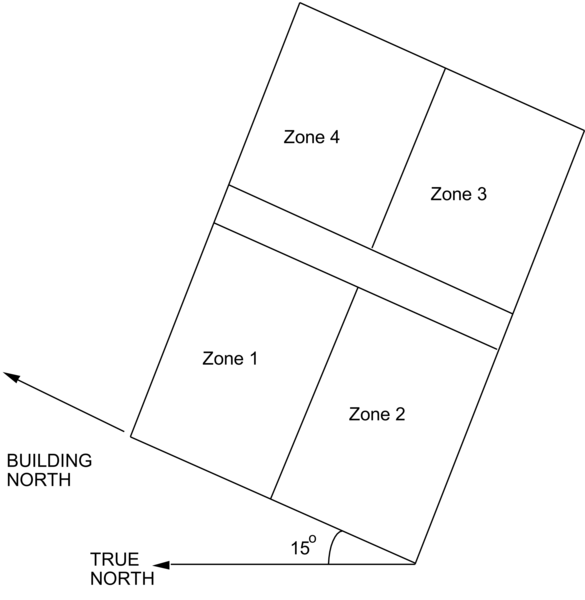
\includegraphics[width=0.4\textwidth, height=0.9\textheight, keepaspectratio=true]{media/image001.png}
    \caption{Illustration of Building North Axis \protect \label{fig:illustration-of-building-north-axis}}
\end{figure}

\paragraph{Field: Terrain}\label{field-terrain}

The site's terrain affects how the wind hits the building -- as does the building height. In addition, the external conduction method usually has its own parameters for the calculation. Please see the Engineering Documentation, External Conduction section for particulars. The legal values for this field are shown in the following table.

% table 1
\begin{longtable}[c]{@{}ll@{}}
    \caption{Values for ``Terrain'' \label{table:values-for-terrain}} \tabularnewline
    \toprule
    Terrain Type Value & Terrain Description \tabularnewline
    \midrule
    \endfirsthead

    \caption[]{Values for ``Terrain''} \tabularnewline
    \toprule
    Terrain Type Value & Terrain Description \tabularnewline
    \midrule
    \endhead

    Country & Flat, Open Country \tabularnewline
    Suburbs & Rough, Wooded Country, Suburbs \tabularnewline
    City & Towns, city outskirts, center of large cities \tabularnewline
    Ocean & Ocean, Bayou flat country \tabularnewline
    Urban & Urban, Industrial, Forest \tabularnewline
    \bottomrule
\end{longtable}

\paragraph{Warmup Convergence}\label{warmup-convergence}

The following two fields along with the minimum and maximum number of warmup days (also in this object) define the user specified criteria for when EnergyPlus will ``converge'' at each environment (each sizing period or run period set as Yes in the \hyperref[simulationcontrol]{SimulationControl} object). At the beginning of a new environment the building model is reinitialized so that temperatures are initialized to 23C and zone humidity ratios are initialized to the outdoor humidity ratio  (unless this initialization is suppressed using the input field called Begin Environment Reset Mode in the \hyperref[sizingperioddesignday]{SizingPerod:DesignDay} object). EnergyPlus repeatedly ``runs'' the first day of the environment or until it reaches ``maximum number of warmup days'' or the convergence criteria are met. Note that setting the convergence tolerance values too loose will cause the program to be satisfied too early and you may not get the results you expect from the actual simulation. However too tight of a value and the program will repeat the first day too many times leading to excessive simulation run time.

\paragraph{Field: Loads Convergence Tolerance Value}\label{field-loads-convergence-tolerance-value}

This value represents the number at which the loads values must agree before ``convergence'' is reached. Loads tolerance is the change in peak zone heating and cooling loads that are predicted from previous warmup day to the current day, in units of W.

\paragraph{Field: Temperature Convergence Tolerance Value}\label{field-temperature-convergence-tolerance-value}

This value represents the number at which the zone temperatures must agree (from previous iteration) before ``convergence'' is reached. (Units for this field is delta C).

Convergence of the simultaneous heat balance/HVAC solution is reached when either the loads or temperature criterion is satisfied.

All tolerances have units so the temperature tolerance is in degrees C (or degrees K) and the loads tolerance is in Watts. Both tolerances work the same way, just one looks at temperatures and one looks at heating and cooling loads. After the second warm-up day, the program compares the maximum temperature experienced in a space with the maximum temperature from the previous day. If those two temperatures are within the tolerance, then it has passed the first warm-up check.

It does a similar comparison with lowest temperatures experience within all the zones. If the current simulation day and the previous day values are within the tolerance, then it has passed the second warm-up check. Similar things are done with the loads tolerance and the maximum heating and cooling loads that are experienced within the spaces. Those are compared individually to the values for the previous day. If they are both in tolerance, then the simulation has passed the third and fourth warm-up check. The simulation stays in the warm-up period until ALL FOUR checks have been passed. See Engineering Reference and Output Details document for further explanation and outputs.

Please note--other ``convergence tolerance'' inputs are required for certain HVAC equipment (unit ventilator, unit heater, window AC, etc.). The purpose and units of these parameters are different from ``load convergence tolerance'' and ``temperature convergence tolerance'' in the BUILDING object.

\paragraph{Field: Solar Distribution}\label{field-solar-distribution}

Setting this value determines how EnergyPlus treats beam solar radiation and reflectances from exterior surfaces that strike the building and, ultimately, enter the zone. There are five choices: \textbf{MinimalShadowing}, \textbf{FullExterior} and \textbf{FullInteriorAndExterior, FullExteriorWithReflections, FullInteriorAndExteriorWithReflections}.

\textbf{MinimalShadowing}

In this case, there is no exterior shadowing except from window and door reveals. All beam solar radiation entering the zone is assumed to fall on the floor, where it is absorbed according to the floor's solar absorptance. Any reflected by the floor is added to the reflected diffuse radiation, which is assumed to be uniformly distributed on all interior surfaces. If no floor is present in the zone, the incident beam solar radiation is absorbed on all interior surfaces according to their absorptances. The zone heat balance is then applied at each surface and on the zone's air with the absorbed radiation being treated as a flux on the surface.

\textbf{FullExterior, FullExteriorWithReflections}

In this case, shadow patterns on exterior surfaces caused by detached shading, wings, overhangs, and exterior surfaces of all zones are computed. As for MinimalShadowing, shadowing by window and door reveals is also calculated. Beam solar radiation entering the zone is treated as for MinimalShadowing -- All beam solar radiation entering the zone is assumed to fall on the floor, where it is absorbed according to the floor's solar absorptance. Any reflected by the floor is added to the reflected diffuse radiation, which is assumed to be uniformly distributed on all interior surfaces. If no floor is present in the zone, the incident beam solar radiation is absorbed on all interior surfaces according to their absorptances. The zone heat balance is then applied at each surface and on the zone's air with the absorbed radiation being treated as a flux on the surface.

\textbf{FullInteriorAndExterior, FullInteriorAndExteriorWithReflections}

This is the same as FullExterior except that instead of assuming all transmitted beam solar falls on the floor the program calculates the amount of beam radiation falling on each surface in the zone, including floor, walls and windows, by projecting the sun's rays through the exterior windows, taking into account the effect of exterior shadowing surfaces and window shading devices.

If this option is used, you should be sure that the surfaces of the zone totally enclose a space. This can be determined by viewing the \textbf{eplusout.dxf} file with a program like AutoDesk's Volo View Express. You should also be sure that the zone is \textbf{convex}. Examples of convex and non-convex zones are shown in Figure~\ref{fig:illustration-of-convex-and-non-convex-zones}. The most common non-convex zone is an L-shaped zone. (A formal definition of convex is that any straight line passing through the zone intercepts at most two surfaces.) If the zone's surfaces do not enclose a space, Solar Distribution should be set to \textbf{FullExterior} instead of \textbf{FullInteriorAndExterior}.  If the zone or a surface in the zone is not convex, Solar Distribution should also be set to \textbf{FullExterior} instead of \textbf{FullInteriorAndExterior} unless this file is not using PolygonClipping (see the \hyperref [field-shading-calculation-method]{Shading Calculation Method} field in \hyperref[shadowcalculation]{ShadowCalculation} for more information).

If you use \textbf{FullInteriorAndExterior} the program will also calculate how much beam radiation falling on the inside of an exterior window (from other windows in the zone) is absorbed by the window, how much is reflected back into the zone, and how much is transmitted to the outside. In this calculation the effect of a shading device, if present, is accounted for.

\begin{figure}[hbtp] % fig 2
    \centering
    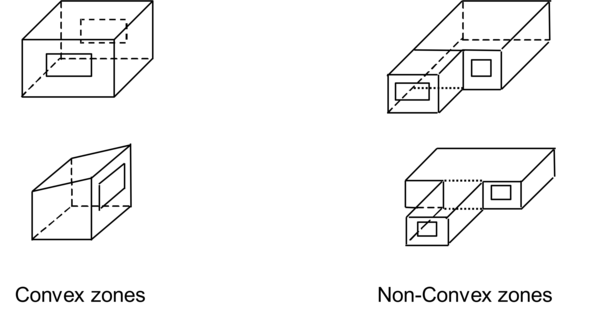
\includegraphics[width=0.9\textwidth, height=0.5\textheight, keepaspectratio=true]{media/image002.png}
    \caption{Illustration of Convex and Non-convex Zones \protect \label{fig:illustration-of-convex-and-non-convex-zones}}
\end{figure}

\textbf{Diffuse Radiation}

Diffuse solar transmitted through exterior and interior windows is distributed according to the approximate view factors between the transmitting window and all other heat transfer surfaces in the zone.
The portion of this diffuse solar that is reflected by all surfaces in the zone is subsequently redistributed uniformly (based on area and solar absorptance) to all heat transfer surfaces in the zone, along with interior reflected beam solar and shortwave radiation from lights. Refer to the section ``Solar Distribution'' in the Engineering Reference Guide for more information including equations.

\textbf{Reflection calculations}

Note: Using the reflection calculations can be very time-consuming. Even error-prone. As a possible alleviation, you can use the \hyperref[outputdiagnostics]{Output:Diagnostics} ``DoNotMirrorDetachedShading'' in many cases to get past a fatal error.

If using reflections, the program calculates beam and sky solar radiation that is reflected from exterior surfaces and then strikes the building. These reflecting surfaces fall into three categories:

1) \textbf{Shadowing surfaces}. These are surfaces like overhangs or neighboring buildings entered with Shad\-ing:\-Site, Shad\-ing:\-Build\-ing, Shad\-ing:\-Site:\-Detailed, Shad\-ing:\-Build\-ing:\-Detailed, Shad\-ing:\-Over\-hang, Shad\-ing:\-Over\-hang:Pro\-jection, Shad\-ing:\-Fin, Shad\-ing:\-Fin:\-Pro\-jection or Shad\-ing:\-Zone:\-Detailed objects. See Figure~\ref{fig:solar-reflection-from-shadowing-surfaces.}.

These surfaces can have diffuse and/or specular (beam-to-beam) reflectance values that are specified with the Shad\-ing\-Property:\-Re\-flectance object which specifies those parameters. They have a default value of .2 for both visible and diffuse reflection.

2) \textbf{Exterior building surfaces}. In this case one section of the building reflects solar radiation onto another section (and vice-versa). See Figure~\ref{fig:solar-reflection-from-building-surfaces-onto}.

The building surfaces are assumed to be diffusely reflecting if they are opaque (walls, for example) and specularly reflecting if they are windows or glass doors. The reflectance values for opaque surfaces are calculated by the program from the Solar Absorptance and Visible Absorptance values of the outer material layer of the surface's construction (ref: Material object properties). The reflectance values for windows and glass doors are calculated by the program from the reflectance properties of the individual glass layers that make up surface's construction assuming no shading device is present and taking into account inter-reflections among the layers (ref: Window Properties).

3) \textbf{The ground surface}. Reflection from the ground is calculated even if reflections option is not used;l but then the ground plane is considered unobstructed, i.e., the shadowing of the ground by the building itself or by obstructions such as neighboring buildings is ignored. Shadowing by the building itself or neighboring buildings is taken into account when the ``with reflections'' option is used but then the ``view factor to ground'' is NOT used. This is shown in Figure~\ref{fig:shadowing-from-building-affects-beam-solar}.

\begin{figure}[hbtp] % fig 3
    \centering
    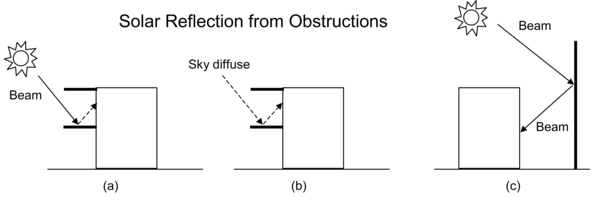
\includegraphics[width=0.9\textwidth, height=0.7\textheight, keepaspectratio=true]{media/image003.png}
    \caption{  Solar reflection from shadowing surfaces. Solid arrows are beam solar radiation; dashed arrows are diffuse solar radiation. (a) Diffuse reflection of beam solar radiation from the top of an overhang. (b) Diffuse reflection of sky solar radiation from the top of an overhang. (c) Beam-to-beam (specular) reflection from the façade of an adjacent highly-glazed building represented by a vertical shadowing surface. \protect \label{fig:solar-reflection-from-shadowing-surfaces.}}
\end{figure}

\begin{figure}[hbtp] % fig 4
    \centering
    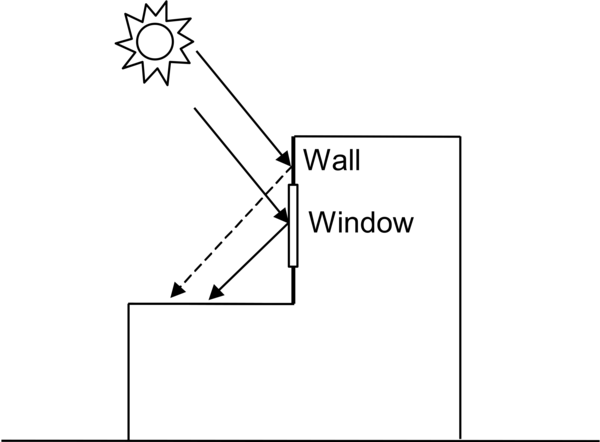
\includegraphics[width=0.9\textwidth, height=0.7\textheight, keepaspectratio=true]{media/image004.png}
    \caption{  Solar reflection from building surfaces onto other building surfaces. In this example beam solar reflects from a vertical section of the building onto a roof section. The reflection from the window is specular. The reflection from the wall is diffuse. \protect \label{fig:solar-reflection-from-building-surfaces-onto}}
\end{figure}

\begin{figure}[hbtp] % fig 5
    \centering
    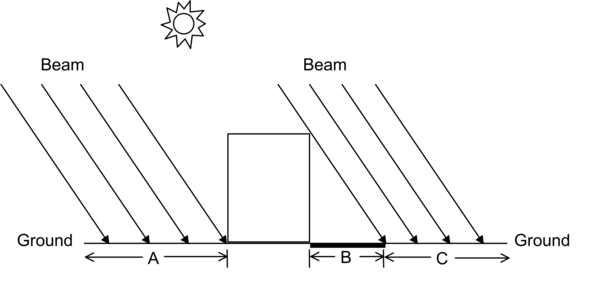
\includegraphics[width=0.9\textwidth, height=0.7\textheight, keepaspectratio=true]{media/image005.png}
    \caption{Shadowing from building affects beam solar reflection from the ground. Beam-to-diffuse reflection from the ground onto the building occurs only for sunlit areas, A and C, not from shaded area, B. \protect \label{fig:shadowing-from-building-affects-beam-solar}}
\end{figure}

\paragraph{Field: Maximum Number of Warmup Days}\label{field-maximum-number-of-warmup-days}

This field specifies the number of ``warmup'' days that might be used in the simulation before ``convergence'' is achieved. The default number, 25, is usually more than sufficient for this task; however, some complex buildings (with complex constructions) may require more days. If you enter less than 25 as a maximum, that is the number of maximum warmup days that will be used. An error message will occur when the simulation ``runs'' out of days and has not converged:

\begin{lstlisting}
CheckWarmupConvergence: Loads Initialization, Zone = "MAIN ZONE" did not converge after 30 warmup days.
See Warmup Convergence Information in .eio file for details
..Environment(SizingPeriod) = "DENVER CENTENNIAL  GOLDEN   N ANN CLG 1% CONDNS DB = >MWB"
..Max Temp Comparison = 2.06E-002 vs Temperature Convergence Tolerance = 0.50 – Pass Convergence
..Min Temp Comparison = 5.95E-003 vs Temperature Convergence Tolerance = 0.50 – Pass Convergence
..Max Cool Load Comparison = 9.5082E-002 vs Loads Convergence Tolerance = 5.00E-002 – Fail Convergence
\end{lstlisting}

As noted in the message, there will be more information in the .eio file. (Refer to Output Details document as well for examples.)

You may be able to increase the Maximum Number of Warmup Days and get convergence, but some anomalous buildings may still not converge. Simulation proceeds for x warmup days until ``convergence'' is reached (see the discussion under the Temperature Convergence Tolerance Value field in this object, just above).

The value in this field is an overall parameter for all types of environments in the simulation. The maximum number of warmup days can also be controlled separately for individual design days using the input field Maximum Number Warmup Days in the \hyperref[sizingperioddesignday]{SizingPerod:DesignDay} object.

\paragraph{Field: Minimum Number of Warmup Days}\label{field-minimum-number-of-warmup-days}

This field specifies the minimum number of ``warmup'' days before EnergyPlus will check if it has achieved convergence and can thus start simulating the particular environment (design day, annual run) in question. Although some older investigations indicated that 6 warmup days is generally enough on the minimum end of the spectrum, current thinking is that the convergence checks (controlled by convergence tolerance values above) can be relied on to determine a minimum number of warm days. An arbitrary high minimum can lead to excessive run times for lightweight buildings that may converge quickly and not need many warmup days. Therefore the default is reduced from 6 to just 1. A value of 6 here will replicate older behavior if field was being left blank. Users may wish to increase the value in certain situations when, based on the output variables described in the Output Details document, it is determined that EnergyPlus has not converged. While this parameter should be less than the previous maximum parameter, a value greater than the value entered in the field ``Maximum Number of Warmup Days'' above may be used when users wish to increase warmup days more than the previous field. In this particular case, the previous field will be automatically reset to the value entered in this field and EnergyPlus will run exactly the number of warmup days specified in this field.

An example from an IDF:

\begin{lstlisting}

Building,
    PSI HOUSE DORM AND OFFICES,  !- Name
    36.87000,               !- North Axis {deg}
    Suburbs,                !- Terrain
    0.04,                   !- Loads Convergence Tolerance Value
    0.4000000,              !- Temperature Convergence Tolerance Value {deltaC}
    FullInteriorAndExterior, !- Solar Distribution
    40,                     !- Maximum Number of Warmup Days
    6;                      !- Minimum Number of Warmup Days
\end{lstlisting}

\subsection{SurfaceConvectionAlgorithm:Inside}\label{surfaceconvectionalgorithminside}

This input object is used control the choice of models used for surface convection at the inside face of all the heat transfer surfaces in the model. This object sets the selection for convection correlations in a global way. The Zone Inside Convection Algorithm input field in the Zone object may be used to selectively override this value on a zone-by-zone basis. Further, individual surfaces can refine the choice by each surface or surface lists -- see object \hyperref[surfacepropertyconvectioncoefficients]{SurfaceProperty:ConvectionCoefficients} and object \hyperref[surfacepropertyconvectioncoefficientsmultiplesurface]{SurfaceProperty:ConvectionCoefficients:MultipleSurface}.

\subsubsection{Inputs}\label{inputs-4-031}

\paragraph{Field: Algorithm}\label{field-algorithm-000}

The model specified in this field is the default algorithm for the inside face all the surfaces.. The key choices are \textbf{Simple}, \textbf{TARP}, \textbf{CeilingDiffuser}, \textbf{AdaptiveConvectionAlgorithm}, and \textbf{ASTMC1340}.

The \textbf{Simple} model applies constant heat transfer coefficients depending on the surface orientation.

The \textbf{TARP} model correlates the heat transfer coefficient to the temperature difference for various orientations. This model is based on flat plate experiments.

The \textbf{CeilingDiffuser} model is a mixed and forced convection model for ceiling diffuser configurations. The model correlates the heat transfer coefficient to the air change rate for ceilings, walls and floors. These correlations are based on experiments performed in an isothermal room with a cold ceiling jet. To avoid discontinuities in surface heat transfer rate calculations, all of correlations have been extrapolated beyond the lower limit of the data set (3 ACH) to a natural convection limit that is applied during the hours when the system is off.

The \textbf{AdaptiveConvectionAlgorithm} model is an dynamic algorithm that organizes a large number of different convection models and automatically selects the one that best applies. The adaptive convection algorithm can also be customized using the \hyperref[surfaceconvectionalgorithminsideadaptivemodelselections]{SurfaceConvectionAlgorithm:Inside:AdaptiveModelSelections} input object. These models are explained in detail in the EnergyPlus Engineering Reference Document.

The \textbf{ASTMC1340} model correlates mixed convection coefficients to the surface-to-air temperature difference, heat flow direction, surface tilt angle, surface characteristic length, and air speed past the surface. These correlations are based on ASTM C1340 standard.

The default is \textbf{TARP}.

IDF Example:

\begin{lstlisting}

SurfaceConvectionAlgorithm:Inside,TARP;
\end{lstlisting}

\subsection{SurfaceConvectionAlgorithm:Outside}\label{surfaceconvectionalgorithmoutside}

Various exterior convection models may be selected for global use. The optional Zone Outside Convection Algorithm input field in the Zone object may be used to selectively override this value on a zone-by-zone basis. Further, individual surfaces can refine the choice by each surface or surface lists -- see object \hyperref[surfacepropertyconvectioncoefficients]{SurfaceProperty:ConvectionCoefficients} and object \hyperref[surfacepropertyconvectioncoefficientsmultiplesurface]{SurfaceProperty:ConvectionCoefficients:MultipleSurface}.

\subsubsection{Inputs}\label{inputs-5-028}

\paragraph{Field: Algorithm}\label{field-algorithm-1-000}

The available key choices are \textbf{SimpleCombined}, \textbf{TARP}, \textbf{MoWiTT}, \textbf{DOE-2}, and \textbf{AdaptiveConvectionAlgorithm}.

The \textbf{Simple} convection model applies heat transfer coefficients depending on the roughness and windspeed. This is a combined heat transfer coefficient that includes radiation to sky, ground, and air. The correlation is based on Figure~\ref{fig:schematic-of-the-energyplus-unitary-system}, Page 25.1 (Thermal and Water Vapor Transmission Data), 2001 ASHRAE Handbook of Fundamentals. Note that if \textbf{Simple} is chosen here or in the Zone field and a \hyperref[surfacepropertyconvectioncoefficients]{SurfaceProperty:ConvectionCoefficients} object attempts to override the calculation with a different choice, the action will still be one of combined calculation. To change this, you must select one of the other methods for the global default.

All other convection models apply heat transfer coefficients depending on the roughness, windspeed, and terrain of the building's location. These are \emph{convection only} heat transfer coefficients; radiation heat transfer coefficients are calculated automatically by the program.

The \textbf{TARP} algorithm was developed for the TARP software and combines natural and wind-driven convection correlations from laboratory measurements on flat plates.

The \textbf{DOE-2} and \textbf{MoWiTT} were derived from field measurements. DOE-2 uses a correlation from measurements by Klems and Yazdanian for rough surfaces. MoWitt uses a correlation from measurements by Klems and Yazdanian for smooth surfaces and, therefore, is most appropriate for windows (see \hyperref[surfacepropertyconvectioncoefficientsmultiplesurface]{SurfaceProperty:ConvectionCoefficients:MultipleSurface} for how to apply to only windows).

The \textbf{AdaptiveConvectionAlgorithm} model is an dynamic algorithm that organizes a large number of different convection models and automatically selects the one that best applies. The adaptive convection algorithm can also be customized using the \hyperref[surfaceconvectionalgorithmoutsideadaptivemodelselections]{SurfaceConvectionAlgorithm:Outside:AdaptiveModelSelections} input object. All algorithms are described more fully in the Engineering Reference.

The default is \textbf{DOE-2}.

Note that when the surface is wet (i.e. it is raining and the surface is exposed to wind) then the convection coefficient appears as a very large number (1000) and the surface is exposed to the Outdoor Wet-bulb Temperature rather than the Outdoor Dry-bulb Temperature.

IDF Example:

\begin{lstlisting}

SurfaceConvectionAlgorithm:Outside, AdaptiveConvectionAlgorithm;
\end{lstlisting}

\subsection{HeatBalanceAlgorithm}\label{heatbalancealgorithm}

The HeatBalanceAlgorithm object provides a way to select what type of heat and moisture transfer algorithm will be used for calculating the performance of the building's surface assemblies. This input controls the overall algorithm used for all the surfaces unless one or more of the SurfaceProperty:HeatTransferAlgorithm:* objects are used to alter the selection for particular surfaces.

\subsubsection{Inputs}\label{inputs-6-025}

\paragraph{Field: Algorithm}\label{field-algorithm-2-000}

Four values are allowed to select which solution will be used.

\begin{itemize}
    \item
    The \textbf{ConductionTransferFunction} selection is a sensible heat only solution and does not take into account moisture storage or diffusion in the construction elements.
    \item
    The \textbf{MoisturePenetrationDepthConductionTransferFunction} selection is a sensible heat diffusion and an inside surface moisture storage algorithm that also needs additional moisture material property information. Sometimes, this is referred to as the Effective Moisture Penetration Depth or EMPD. See the moisture material property object for additional information and description of outputs:
    \begin{itemize}
        \item
        \hyperref[materialpropertymoisturepenetrationdepthsettings]{MaterialProperty:MoisturePenetrationDepth:Settings}
    \end{itemize}
    \item
    \textbf{Advanced/Research usage:}The \textbf{ConductionFiniteDifference} selection is a sensible heat only solution and does not take into account moisture storage or diffusion in the construction elements. This solution technique uses a 1-D finite difference solution in the construction elements. Outputs for the surfaces are described with the material property objects. The Conduction Finite Difference (aka CondFD) property objects are:
    \begin{itemize}
        \item
        \hyperref[materialpropertyphasechange]{MaterialProperty:PhaseChange}
        \item
        \hyperref[materialpropertyvariablethermalconductivity]{MaterialProperty:VariableThermalConductivity}
        \item
        \hyperref[materialpropertyphasechangehysteresis]{MaterialProperty:PhaseChangeHysteresis}
    \end{itemize}
    \item
    \textbf{Advanced/Research usage:} The \textbf{CombinedHeatAndMoistureFiniteElement} is a coupled heat and moisture transfer and storage solution. The solution technique uses a one dimensional finite difference solution in the construction elements and requires further material properties described in the Heat and Moisture Transfer material properties objects. Outputs from the algorithm are described with these objects. The Heat and Moisture Transfer property objects are:
    \begin{itemize}
        \item
        \hyperref[materialpropertyheatandmoisturetransfersettings]{MaterialProperty:HeatAndMoistureTransfer:Settings}
        \item
        \hyperref[materialpropertyheatandmoisturetransfersorptionisotherm]{MaterialProperty:HeatAndMoistureTransfer:SorptionIsotherm}
        \item
        \hyperref[materialpropertyheatandmoisturetransfersuction]{MaterialProperty:HeatAndMoistureTransfer:Suction}
        \item
        \hyperref[materialpropertyheatandmoisturetransferredistribution]{MaterialProperty:HeatAndMoistureTransfer:Redistribution}
        \item
        \hyperref[materialpropertyheatandmoisturetransferdiffusion]{MaterialProperty:HeatAndMoistureTransfer:Diffusion}
        \item
        \hyperref[materialpropertyheatandmoisturetransferthermalconductivity]{MaterialProperty:HeatAndMoistureTransfer:ThermalConductivity}
    \end{itemize}
\end{itemize}

\paragraph{Field: Surface Temperature Upper Limit}\label{field-surface-temperature-upper-limit}

This field is a bit ``advanced''. It should only be used when the simulation fails AND you cannot determine a cause for the failure. That is, you receive an error similar to:

\begin{lstlisting}
   ** Severe  ** Temperature out of bounds (202.91) for surface = Wall1
   **   ~~~   ** in Zone = Zone01
   **   ~~~   **  Occurrence info = NEW YORK CITY NY SUMMER, 07/21 16:00 - 16:01
   **   ~~~   ** A temperature out of bounds problem can be caused by several things.  The user
   **   ~~~   ** should check the weather environment, the level of internal gains with respect
   **   ~~~   ** to the zone, and the thermal properties of their materials among other things.
   **   ~~~   ** A common cause is a building with no thermal mass -- all materials with
   **   ~~~   ** Regular-R definitions.
\end{lstlisting}

And, after careful perusal, you cannot find a solution as suggested in the error description. You may then want to enter a higher number than the default for this field.

\paragraph{Field: Minimum Surface Convection Heat Transfer Coefficient Value}\label{field-minimum-surface-convection-heat-transfer-coefficient-value}

This optional field is used to set an overall minimum for the value of the coefficient for surface convection heat transfer (Hc) in W/m2-K. A minimum is necessary for numerical robustness because some correlations for Hc can result in zero values and create numerical problems. This field can be used to support specialized validation testing to suppress convection heat transfer and to investigate the implications of different minimum Hc values. The default is 0.1.

\paragraph{Field: Maximum Surface Convection Heat Transfer Coefficient Value}\label{field-maximum-surface-convection-heat-transfer-coefficient-value}

This optional field is used to set an overall maximum for the value of the coefficient for surface convection heat transfer (Hc) in W/m2-K. High Hc values are used in EnergyPlus to approximate fixed surface temperature boundary conditions. This field can be used to alter the accepted range of user-defined Hc values.

And, a default IDF example

\begin{lstlisting}
HeatBalanceAlgorithm,ConductionTransferFunction; ! Solution Algorithm
\end{lstlisting}

\subsection{HeatBalanceSettings:ConductionFiniteDifference}\label{heatbalancesettingsconductionfinitedifference}

This object is used to control the behavior of the Conduction Finite Difference algorithm for surface heat transfer. The settings are global and affect how the model behaves for all the surfaces.

\subsubsection{Inputs}\label{inputs-7-025}

\paragraph{Field: Difference Scheme}\label{field-difference-scheme}

This field determines the solution scheme used by the Conduction Finite Difference model. There are two options CrankNicholsonSecondOrder and FullyImplicitFirstOrder. The CrankNicholsonSecondOrder scheme is second order in time and may be faster. But it can be unstable over time when boundary conditions change abruptly and severely. The FullyImplicitFirstOrder scheme is first order in time and is more stable over time. But it may be slower. The default is FullyImplicitFirstOrder when ConductionFiniteDifference is selected as the Heat Balance Algorithm.

\paragraph{Field: Space Discretization Constant}\label{field-space-discretization-constant}

This field controls how the model determines spatial discretization, or the count of nodes across each material layer in the construction. The model calculates the nominal distance associated with a node, \(\Delta x\), using

\begin{equation}
    \Delta x = \sqrt {C\alpha \Delta t}
\end{equation}

Where

\(\alpha\) is the thermal diffusivity of the material layer, in m\(^{2}\)/s

\(\Delta t\) is the length of the timestep in seconds.

\emph{C} is a constant set by this field.

The default is 3. Typical values are from 1 to 3. Lower values for this constant lead to more nodes and finer-grained space discretization.

\paragraph{Field: Relaxation Factor}\label{field-relaxation-factor}

The finite difference solver includes under-relaxation for improved stability for interactions with the other surfaces. This input field can optionally be used to modify the starting value for the relaxation factor. Larger numbers may solve faster, while smaller numbers may be more stable. The default is 1.0. If the program detects numerical instability, it may reduce the value entered here to something lower and more stable.

\paragraph{Field: Inside Face Surface Temperature Convergence Criteria}\label{field-inside-face-surface-temperature-convergence-criteria}

The surface heat balance model at the inside face has a numerical solver that uses a convergence parameter for a maximum allowable differences in surface temperature. This field can optionally be used to modify this convergence criteria. The default value is 0.002 and was selected for stability. Lower values may further increase stability at the expense of longer runtimes, while higher values may decrease runtimes but lead to possible instabilities. The units are in degrees Celsius.

An example IDF object follows.

\begin{lstlisting}
HeatBalanceSettings:ConductionFiniteDifference,
  FullyImplicitFirstOrder, !- Difference Scheme
  3.0,                     !- Space Discretization Constant
  1.0,                     !- Relaxation Factor
  0.002;                   !- Inside Face Surface Temperature Convergence Criteria
\end{lstlisting}

\subsection{ZoneAirHeatBalanceAlgorithm}\label{zoneairheatbalancealgorithm}

The ZoneAir\hyperref[heatbalancealgorithm]{HeatBalanceAlgorithm} object provides a way to select what type of solution algorithm will be used to calculate zone air temperatures and humidity ratios. This object is an optional object. If the default algorithm is used, this object is not required in an input file.

\subsubsection{Inputs}\label{inputs-8-023}

\paragraph{Field: Algorithm}\label{field-algorithm-3-000}

Three choices are allowed to select which solution algorithm will be used. The \textbf{ThirdOrderBackwardDifference} selection is the default selection and uses the third order finite difference approximation to solve the zone air energy and moisture balance equations. The \textbf{AnalyticalSolution} selection uses the integration approach to solve the zone air energy and moisture balance equations. The \textbf{EulerMethod} selection uses the first order finite backward difference approximation to solve the zone air energy and moisture balance equations.

\paragraph{Field: Do Space Heat Balance for Sizing}\label{field-do-space-heat-balance-sizing}
If yes, space-level heat balance will be calculated and reported during sizing, and space sizing results will be reported along with zone sizing results. If no, then only zone-level heat balance will be calculated. This field defaults to No. For zones with more than one space, the zone sizing results are calculated for the whole zone and represent the coincident peak for the spaces in the zone. Note that space heat balance is not supported for \hyperref[inputs-hm]{HybridModel:Zone}, \hyperref[roomairmodeltype]{RoomAirModelType} other than Mixing, \hyperref[heatbalancealgorithm]{HeatBalanceAlgorithm} MoisturePenetrationDepthConductionTransferFunction and CombinedHeatAndMoistureFiniteElement.

\paragraph{Field: Do Space Heat Balance for Simulation}\label{field-do-space-heat-balance-simulation}
If yes, space-level heat balance will be calculated and reported during the simulation. If no, then only zone-level heat balance will be calculated. This field defaults to No. When this field is Yes, optional SpaceHVAC objects may be used to distribute zone HVAC equipment output to the spaces in the zone. See \hyperref[spacehvacequipmentconnections]{SpaceHVAC:EquipmentConnections}, \hyperref[spacehvaczoneequipmentsplitter]{SpaceHVAC:ZoneEquipmentSplitter} and \hyperref[spacehvaczoneequipmentmixer]{SpaceHVAC:ZoneEquipmentMixer}.

And, a default IDF example is shown below:

\begin{lstlisting}
ZoneAirHeatBalanceAlgorithm, ThirdOrderBackwardDifference; !- Algorithm
\end{lstlisting}

\subsection{ZoneAirContaminantBalance}\label{zoneaircontaminantbalance}

The ZoneAirContaminantBalance object provides a way to select which contaminant type will be simulated. Although carbon dioxide is not considered as an indoor contaminant but it is used as an indicator of indoor air quality in buildings. From modeling point of view EnergyPlus treats carbon dioxide as a type of contaminant. In addition to carbon dioxide, a generic contaminant type model was also added. This object is optional, only required in the input data file if the user wishes to model contaminant concentration levels as part of their simulation.

\subsubsection{Inputs}\label{inputs-9-021}

\paragraph{Field: Carbon Dioxide Concentration}\label{field-carbon-dioxide-concentration}

Input is Yes or No. The default is No. If Yes, simulation of carbon dioxide concentration levels will be performed. If No, simulation of carbon dioxide concentration levels will not be performed.

\paragraph{Field: Outdoor Carbon Dioxide Schedule Name}\label{field-outdoor-carbon-dioxide-schedule-name}

This field specifies the name of a schedule that contains outdoor air carbon dioxide level values in units of ppm. One source of monthly average CO\(_{2}\) levels in the atmosphere is available at \href{http://www.esrl.noaa.gov/gmd/ccgg/trends/}{NOAA's website} or via \href{ftp://aftp.cmdl.noaa.gov/products/trends/co2/co2_mm_mlo.txt}{ftp}.

\paragraph{Field: Generic Contaminant Concentration}\label{field-generic-contaminant-concentration}

Input is Yes or No. The default is No. If Yes, simulation of generic contaminant concentration levels will be performed. If No, simulation of generic contaminant concentration levels will not be performed.

\paragraph{Field: Outdoor Generic Contaminant Schedule Name}\label{field-outdoor-generic-contaminant-schedule-name}

This field specifies the name of a schedule that contains outdoor air generic contaminant level values in units of ppm.

An IDF example:

\begin{lstlisting}
ZoneAirContaminantBalance,
  Yes,                          !- Carbon Dioxide Concentration
  Outdoor CO2 Schedule,         !- Outdoor Carbon Dioxide Schedule Name
  Yes,                          !- Generic Contaminant Concentration
  Generic Contaminant Schedule; !- Outdoor Generic Contaminant Schedule Name
\end{lstlisting}

\subsubsection{Outputs}\label{outputs-033}

The following output variables are available when Carbon Dioxide Concentration = Yes.

\begin{lstlisting}
HVAC,Average,Zone Air CO2 Internal Gain Volume Flow Rate [m3/s]
HVAC,Average,Zone Air CO2 Concentration [ppm]
\end{lstlisting}

\paragraph{Zone Air CO2 Concentration {[}ppm{]}}\label{zone-air-co2-concentration-ppm}

This output variable represents the carbon dioxide concentration level in parts per million (ppm) for each zone. This is calculated and reported from the Correct step in the Zone Air Contaminant Predictor-Corrector module.

\paragraph{Zone Air CO2 Internal Gain Volume Flow Rate {[}m3/s{]}}\label{zone-air-co2-internal-gain-volume-flow-rate-m3s}

This is the total (net) rate of carbon dioxide internal gains/losses for a zone in \si{\volumeFlowRate} from all types of sources or sinks. It includes impacts from three objects: ZoneContaminantSourceAndSink:CarbonDioxide, People, and GasEquipment. Positive values denote carbon dioxide generation (gain or source), while negative values denote carbon dioxide removal (loss or sink).

\subsubsection{Outputs}\label{outputs-1-024}

The following output variable is available when Generic Contaminant Concentration = Yes.

HVAC,Average,Zone Generic Air Contaminant Generation Volume Flow Rate {[}m3/s{]}

HVAC,Average,Zone Air Generic Air Contaminant Concentration {[}ppm{]}

\paragraph{Zone Air Generic Air Contaminant Concentration {[}ppm{]}}\label{zone-air-generic-air-contaminant-concentration-ppm}

This output variable represents the generic contaminant concentration level in parts per million (ppm) for each zone. This is calculated and reported from the Correct step in the Zone Air Contaminant Predictor-Corrector module.

\paragraph{Zone Generic Air Contaminant Generation Volume Flow Rate {[}m3/s{]}}\label{zone-generic-air-contaminant-generation-volume-flow-rate-m3s}

This is the rate of generic air contaminant added (or subtracted) to a zone from all types of sources or sinks.

\subsection{ShadowCalculation}\label{shadowcalculation}

This object is used to control some details of EnergyPlus's solar, shadowing and daylighting models. There are two basic methods available for the calculations. In order to speed up the calculations, shadowing calculations (sun position, etc.) for the default method are performed over a period of days. Note that this value may be very important for determining the amount of sun entering your building and by inference the amount of cooling or heating load needed for maintaining the thermostatic setpoint temperature(s) of the building. Though termed ``shadowing'' calculations, it in effect determines the sun position for a particular day in a weather file period simulation. (Each design day will use the date of the design day object.) Even though weather file data contains the amount of solar radiation, the internal calculation of sun position will govern how that affects various parts of the building. By default, the calculations are done for every 20 days throughout a weather run period; an average solar position is chosen and the solar factors (such as sunlit areas of surfaces) remain the same for that number of days. When more integrated calculations are needed for controlling dynamic windows or shades, a second method is available where solar calculations are performed at each zone timestep.

This object also allows setting up global flags to import and export exterior shading calculations results. This enables importing pre-calculated results of the shading fractions for each exterior building surface from external simulation tools. This also enables reusing the shading results for parametric runs which usually do not change external shading.

The object also allows input to disable self-shading effect from exterior surfaces from all zones, or from a subset of zones. Two flags are defined to enable the maximal flexibility of various interpretation of self-shading: one to disable shading between zones of a same zone group, the other to disable shading between different zone groups. The shading by exterior surfaces of the specified zones groups will be bypassed.

\subsubsection{Inputs}\label{inputs-10-019}

\paragraph{Field: Shading Calculation Method}\label{field-shading-calculation-method}

Select between CPU-based polygon clipping method, the GPU-based pixel counting method, or importing from external shading data.

Choices are:
\begin{enumerate}
    \item PolygonClipping (default)
    \item PixelCounting
    \item Scheduled
    \item Imported
\end{enumerate}

If \textbf{PixelCounting} is selected and GPU hardware (or GPU emulation) is not available, a warning will be displayed and EnergyPlus will revert to PolygonClipping. Unlike PolygonClipping, PixelCounting has no limitations related to zone concavity when used with any ``FullInterior'' solar distribution options (i.e., it can accommodate both concave and convex zones and surfaces equally).

Use of the PixelCounting method requires some overhead in passing instructions between the CPU and the GPU. For low numbers of shading surfaces (less than about 200 for most hardware), PolygonClipping requires less runtime than PixelCounting. However, PixelCounting runtime scales significantly better at higher numbers of shading surfaces.

Some computers have multiple GPUs. In this case, the highest performance GPU is not always used by default. You may want to select which GPU is used when running EnergyPlus by setting the graphics performance preferences on your computer.

If \textbf{Scheduled} is chosen, the Sunlit Fraction Schedule Name is required in \textbf{\hyperref[surfacePropertylocalEnvironment]{SurfaceProperty:LocalEnvironment}}. The values entered using this schedule name are then used to determine what the fraction of the surface referenced by the SurfaceProperty:LocalEnvironment input is sunlit. If any surfaces does not have their \textbf{\hyperref[surfacePropertylocalEnvironment]{SurfaceProperty:LocalEnvironment}} objects or no schedule is assigned in the Sunlit Fraction Schedule Name field, no shading is assigned on those surfaces or, in other words, the surface is assumed to be in full sun (sunlit fraction equal to 1).

If \textbf{Imported} is chosen, the \textbf{\hyperref[schedulefileshading]{Schedule:File:Shading}} object is required to define the external file that stores all shading calculation results. The results are imported altogether by reading the \textbf{\hyperref[schedulefileshading]{Schedule:File:Shading}} object during initialization. The file explicitly defines the mappings to the surfaces. If the data for a surface is not listed in the file, no shading is assigned on this surface.

The sunlit fraction to overwrite accounts for the shading of both direct and sky diffuse solar radiation caused by all exterior shadowing surfaces. In this case, shadow patterns on exterior surfaces caused by detached shading, side-fins, overhangs, and exterior surfaces of all zones are overwritten. The interior shading devices, such as window shades and blinds, should be further calculated and applied after the importing.

\paragraph{Field: Shading Calculation Update Frequency Method}\label{field-calculation-method-000}

This field is used to control how the solar, shading, and daylighting models are calculated with respect to the time of calculations during the simulation. The default and fastest method is selected using the keyword Periodic. A more detailed and slower method can be selected using the keyword Timestep. The Timestep method must be used for modeling dynamic fenestration and shading surfaces.

\paragraph{Field: Shading Calculation Update Frequency}\label{field-calculation-frequency}

This numeric field will cause the shadowing calculations to be done periodically using the number in the field as the number of days in each period. This field is only used if the default Periodic calculation frequency method is used in the previous field. Using this field will allow you to synchronize the shadowing calculations with changes in shading devices. Using the default of 20 days in each period is the average number of days between significant changes in solar position angles. For these shadowing calculations, an ``average'' (over the time period) of solar angles, position, equation of time are also used.

\paragraph{Field: Maximum Figures in Shadow Overlap Calculations}\label{field-maximum-figures-in-shadow-overlap-calculations}

This numeric field will allow you to increase the number of figures in shadow overlaps in the PolygonClipping method. Due to the shadowing algorithm, the number of shadows in a figure may grow quite large even with fairly reasonable looking structures. Of course, the inclusion of more allowed figures will increase calculation time. Likewise, too few figures may not result in as accurate calculations as you desire.

\paragraph{Field: Polygon Clipping Algorithm}\label{field-polygon-clipping-algorithm}

This is an advanced feature. Prior to V7, the internal polygon clipping method was a special case of the Weiler-Atherton method. Now, three options are available:

\begin{description}
    \item[SutherlandHodgman] A simpler algorithm but it works well in cases where receiving surfaces (of shadows) are non-convex.
    \item[ConvexWeilerAtherton] Only accurate where both casting and receiving surfaces are convex. Warnings/severe errors are displayed when necessary.
    \item[SlaterBarskyandSutherlandHodgman] Slater-Barsky only applies to rectangular surfaces. Polygon clipping for rectangular surfaces will be calculated using the Slater-Barsky algorithm, while the rest adopts the default Sutherl-Hodgman algorithm.
\end{description}

Default is SutherlandHodgman. More details on polygon clipping are contained in the Engineering Reference.

\paragraph{Field: Pixel Counting Resolution}

Number of pixels in both dimensions of the surface rendering. Higher resolution will create more accurate calculations, but can significantly increase computation time.

Default: 512.

\paragraph{Field: Sky Diffuse Modeling Algorithm}\label{field-sky-diffuse-modeling-algorithm}

Two choices are available here: SimpleSkyDiffuseModeling and DetailedSkyDiffuseModeling. \textbf{SimpleSkyDiffuseModeling} (default) performs a one-time calculation for sky diffuse properties. This has implications if you have shadowing surfaces with changing transmittance (i.e. not all opaque or not all transparent) during the year. The program checks to see if this might be the case and automatically selects \textbf{DetailedSkyDiffuseModeling} if the shading transmittance varies. Even if the transmittance doesn't vary and the option for detailed modeling is used, that option is retained (though it will increase execution time) because you may be using EMS to vary the transmittance. When the detailed modeling is done, there will be a warning posted if the Calculation Frequency (above) is \textgreater{} 1.

In general (and you should also read the previous field description), if shadowing surfaces are used with the transmittance property, the user should be careful to synchronize this calculation with the scheduled occurrence of the transmittance (if any) (or use 1, which will be the most accurate but will cause more time in the calculations).

This field applies to the shading calculation update frequency method called ``Periodic.'' When the method called ``Timestep'' is used the diffuse sky modeling always uses DetailedSkyDiffuseModeling.

\paragraph{Field: Output External Shading Calculation Results}\label{field-output-external-shading-calculation results}
This fields indicates whether or not (\textbf{Yes} or \textbf{No})to save internal shading calculation results to an external file, which can be imported back as needed. This file saves external sunlit fractions for all surfaces. If \textbf{Yes} is chosen, hourly shading fraction of all surfaces will be exported as a CSV file, naming as "output file prefix + shading" (the default name is "eplusshading.csv" if no output file prefix is defined). Each column of the CSV file lists the annually calculated shading fraction of each surface with time-step interval. It only writes data for each simulation day that shadows are calculated, e.g. once every 20 days by default. If the results are intended to be reused to be imported back using \textbf{Imported} in \textbf{\hyperref[field-shading-calculation-method]{Field: Shading Calculation Method}}, the Calculation Frequency should be set as one to write year-round hourly results. Design days are not included. The default choice is \textbf{No}.

\paragraph{Field: Disable Self-Shading Within Shading Zone Groups}\label{fieldself--disable-shading-within-a-zone-group}
This fields specifies during shading calculation, for all surfaces in a targeted Zone Group, whether or not (\textbf{Yes} or \textbf{No} ) the self-shading effect by exterior surfaces of all zones within the target Zone Group is disabled. If Yes, self-shading will be disabled from all exterior surfaces in a given Shading Zone Group to surfaces within the same Shading Zone Group. If both Disable Self-Shading Within Shading Zone Groups and Disable Self-Shading From Shading Zone Groups to Other Zones = Yes, then all self-shading from exterior surfaces will be disabled.If only one of these fields = Yes, then at least one Shading Zone Group must be specified, or this field will be ignored. Shading from Shading:* surfaces, overhangs, fins, and reveals will not be disabled.

\paragraph{Field: Disable Self-Shading From Shading Zone Groups to Other Zones}\label{field-self-disable-shading-between-zone-groups}
This fields specifies during shading calculation, for all surfaces in a targeted Zone Group, whether or not (\textbf{Yes} or \textbf{No} ) the self-shading effect from all exterior surfaces in the target Zone Group to other zones is disabled. If Yes, self-shading will be disabled from all exterior surfaces in a given Shading Zone Group to all other zones in the model. If both Disable Self-Shading Within Shading Zone Groups and Disable Self-Shading From Shading Zone Groups to Other Zones = Yes, then all self-shading from exterior surfaces will be disabled. If only one of these fields = Yes, then at least one Shading Zone Group must be specified, or this field will be ignored. Shading from Shading:* surfaces, overhangs, fins, and reveals will not be disabled.

\paragraph{Field: Shading Zone Group ZoneList Name}\label{field-shading-zone-group-zoneList-name}
The shading zones group specifies group of zones which are controlled by the Disable Self-Shading fields. This object is extensible, so additional fields of this type can be added to the end of this object.

Examples of this object in IDF: (note this object must be unique in an IDF)

\begin{lstlisting}
ShadowCalculation, PixelCounting, Periodic, 1;

ShadowCalculation, PolygonClipping, Periodic, 1, , SutherlandHodgman, , DetailedSkyDiffuseModeling;

ShadowCalculation, Scheduled, Periodic, , , , , Yes;

ShadowCalculation, PolygonClipping, Periodic, , , , , , , Yes, No, ShadingZoneGroup;
\end{lstlisting}

Note that the use of ``1'' in the examples is NOT the same as using Timestep calculation frequency -- ``1'' causes daily calculation of the sun position variables but does not change the shadowing calculations more frequently than daily.

\subsection{Output:Diagnostics}\label{outputdiagnostics}

Sometimes, messages only confuse users -- especially new users. Likewise, sometimes certain output variables exist for only a certain condition but some take them at face value/name. Some features may be very important but under certain instances cause problems. Thus, we have added the \textbf{diagnostic output} object to be able to turn on or off certain messages, variables, and features depending on conditions.

Both fields of the Output:Diagnostics command can accept all the applicable keys. More than one object may be entered.

\subsubsection{Inputs}\label{inputs-11-018}

\paragraph{Field: key1, key2}\label{field-key1-key2}

Allowable choices are:

\textbf{DisplayAllWarnings} -- use this to get all warnings (except the developer warnings ``DisplayZoneAirHeatBalanceOffBalance''). This key sets all other display warning values to on.

\textbf{DisplayExtraWarnings} -- use this to get all extra warnings. An example of an extra warning is when a user enters a ceiling height or volume with the Zone object and EnergyPlus calculates something significantly different based on the entered zone geometry.

\textbf{DisplayUnusedSchedules} -- use this to have the unused schedules (by name) listed at the end of the simulation.

\textbf{DisplayUnusedObjects} -- use this to have unused (orphan) objects (by name) listed at the end of the simulation.

\textbf{DisplayAdvancedReportVariables} -- use this to be able to use certain advanced output variables where the name may be misleading and you need to understand the concepts or reasons for use. If you put in this field, then you will be able to report on these features. They are noted in the descriptions of objects or output variables.

\textbf{DisplayZoneAirHeatBalanceOffBalance} -- this is a developer diagnostic which you can turn on, if you desire.

\textbf{DoNotMirrorDetachedShading} -- use this to turn off the automatic mirroring of detached shading surfaces. These surfaces are automatically mirrored so that the user does not need to worry about facing direction of the surface and the shading surface will shade the building as appropriate.

\textbf{DoNotMirrorAttachedShading} -- use this to turn off the automatic mirroring of attached shading surfaces. These surfaces are automatically mirrored so that the user does not need to worry about facing direction of the surface and the shading surface will shade the building as appropriate. Attached shading surfaces include \hyperref[shadingoverhang]{Shading:Overhang}, \hyperref[shadingoverhangprojection]{Shading:Overhang:Projection}, \hyperref[shadingfin]{Shading:Fin}, \hyperref[shadingfinprojection]{Shading:Fin:Projection}, and \hyperref[shadingzonedetailed-000]{Shading:Zone:Detailed}.

\textbf{DisplayWeatherMissingDataWarnings} -- use this to turn on the missing data warnings from the read of the weather file.

\textbf{ReportDuringWarmup} -- use this to allow reporting during warmup days. This can show you exactly how your facility is converging (or not) during the initial ``warmup'' days of the simulation. Generally, only developers or expert simulation users would need this kind of detail.

\textbf{ReportDetailedWarmupConvergence} -- use this to produce detailed reporting (essentially each warmup day for each zone) for warmup convergence.

\textbf{ReportDuringHVACSizingSimulation} -- use this to allow controlling reporting to SQLite database during sizing period simulations done for HVAC Sizing Simulation. The regular reporting is done in the usual way. This can show details of how advanced sizing adjustments were determined by documenting how the systems operated when doing the intermediate sizing periods. Depending on the number of iterations performed for HVAC Sizing Simulation, there will be a number of sets of results with each set containing all the Sizing Periods.

In IDF use:

\begin{lstlisting}
Output:Diagnostics,
  DisplayExtraWarnings;
\end{lstlisting}

\subsection{Output:DebuggingData}\label{outputdebuggingdata}

There may be times when a particular input file requires additional debugging. The Output:DebuggingData object may be used to report all available node data (e.g., temperature, mass flow rate, set point, pressure, etc.). The debug data is reported to the DBG text file. The debug file first reports the node number and name, and then all available node information for each zone time step (Ref. Timestep). Only one object may be entered.

\subsubsection{Inputs}\label{inputs-12-017}

\paragraph{Field: Report Debugging Data}\label{field-report-debugging-data}

This field turns on debug reporting when ``Yes'' is entered. ``No'' (the default) disables debug reporting.

\paragraph{Field: Report During Warmup}\label{field-report-during-warmup}

This field reports the debug data during the warmup period when ``Yes'' is entered. ``No'' (the default) disables reporting during warmup.

In IDF use:

\begin{lstlisting}
Output:DebuggingData,
  Yes,Yes;
\end{lstlisting}

\subsection{Output:PreprocessorMessage}\label{outputpreprocessormessage}

The Output:PreprocessorMessage object can be used by preprocessor programs to EnergyPlus for passing certain conditions/errors that might not be detected by scripts executing the EnergyPlus system of programs. This allows EnergyPlus to intercept problems and terminate gracefully rather than the user having to track down the exact conditions.

There is no reason for a user to enter an Output:PreprocessorMessage object but you should encourage interface developers to use this feature. More than one Output:PreprocessorMessage objects may be entered. Of course, no preprocessor message objects are necessary if there is no error information to be passed.

\subsubsection{Inputs}\label{inputs-13-014}

\paragraph{Field: Preprocessor Name}\label{field-preprocessor-name}

The preprocessor name (e.g. EPMacro, ExpandObjects) is entered here. Case is retained so that messages from EnergyPlus look very similar to what a preprocessor would produce.

\paragraph{Field: Error Severity}\label{field-error-severity}

This is the error severity. If Fatal, EnergyPlus will terminate after showing all preprocessor messages.

\paragraph{Fields: Message Line 1 through Message Line 10}\label{fields-message-line-1-through-message-line-10}

Each line is limited to 100 characters and an appropriate message can be composed.

An IDF Example:

\begin{lstlisting}

Output:PreprocessorMessage,
     No Preprocessor Used,     !- preprocessor name
     Information,              !- error severity
     Illustrative Message,     !- message line 1
     No problems for processing;  !- message line 2
\end{lstlisting}

And would appear in output:

\begin{lstlisting}
Preprocessor = "No Preprocessor Used" has the following Information messages:
Illustrative Message
No problems for processing
\end{lstlisting}

\subsection{ZoneCapacitanceMultiplier:ResearchSpecial}\label{zonecapacitancemultiplierresearchspecial}

This object is an advanced feature that can be used to control the effective storage capacity of the zone. Capacitance multipliers of 1.0 indicate the capacitance is that of the (moist) air in the volume of the specified zone. This multiplier can be increased if the zone air capacitance needs to be increased for stability of the simulation or to allow modeling higher or lower levels of damping of behavior over time. The multipliers are applied to the base value corresponding to the total capacitance for the zone's volume of air at current zone (moist) conditions.

\subsubsection{Inputs}\label{inputs-14-014}

\paragraph{Field: Name}\label{field-name-hybrid-model}

The name of the ZoneCapacitanceMultiplier:ResearchSpecial object.

\paragraph{Field: Zone or ZoneList Name}\label{field-Zone-or-zonelist-name-hybrid-model}

This field is the name of the thermal zone (ref: Zone) and attaches a particular zone capacitance multiplier to a thermal zone or set of thermal zones in the building. When the \hyperref[zonelist]{ZoneList} option is used then capacity multiplier is applied to each of the zones in the zone list.

\paragraph{Field: Temperature Capacity Multiplier}\label{field-temperature-capacity-multiplier}

This field is used to alter the effective heat capacitance of the zone air volume. This affects the transient calculations of zone air temperature. Values greater than 1.0 have the effect of smoothing or damping the rate of change in the temperature of zone air from timestep to timestep. Note that sensible heat capacity can also be modeled using internal mass surfaces.

\paragraph{Field: Humidity Capacity Multiplier}\label{field-humidity-capacity-multiplier}

This field is used to alter the effective moisture capacitance of the zone air volume. This affects the transient calculations of zone air humidity ratio. Values greater than 1.0 have the effect of smoothing, or damping, the rate of change in the water content of zone air from timestep to timestep.

\paragraph{Field: Carbon Dioxide Capacity Multiplier}\label{field-carbon-dioxide-capacity-multiplier}

This field is used to alter the effective carbon dioxide capacitance of the zone air volume. This affects the transient calculations of zone air carbon dioxide concentration. Values greater than 1.0 have the effect of smoothing or damping the rate of change in the carbon dioxide level of zone air from timestep to timestep.

\paragraph{Field: Generic Contaminant Capacity Multiplier}\label{field-generic-contaminant-capacity-multiplier}

This field is used to alter the effective generic contaminant capacitance of the zone air volume. This affects the transient calculations of zone air generic contaminant concentration. Values greater than 1.0 have the effect of smoothing or damping the rate of change in the generic contaminant level of zone air from timestep to timestep.

\subsection{SimulationControl}\label{simulationcontrol}

The input for SimulationControl allows the user to specify what kind of calculations a given EnergyPlus simulation will perform. For instance the user may want to perform one or more of the sizing calculations but not proceed to an annual weather file simulation. Or the user might have all flow rates and equipment sizes already specified and desire an annual weather without any preceding sizing calculations. Sizing runs, even for large projects, are quickly run -- they do not add much to the overall simulation time. The SimulationControl input allows all permutations of run selection by means of 5 yes/no inputs.

\begin{callout}
    Only one SimulationControl object is permitted for each EnergyPlus input file. While a SimulationControl is needed to trigger sizing calculations, it is optional for other runs (design days, run periods). The actions will still be shown in the eplusout.eio file (see Output Details and Examples Document).
\end{callout}

\subsubsection{Inputs}\label{inputs-15-014}

\paragraph{Field: Do Zone Sizing Calculation}\label{field-do-zone-sizing-calculation}

Input is Yes or No. The default is No. Zone Sizing (see \hyperref[sizingzone]{Sizing:Zone} object) performs a special calculation, using a theoretical ideal zonal system, and determines the zone design heating and cooling flow rates and loads, saving the results in the zone sizing arrays.

\paragraph{Field: Do System Sizing Calculation}\label{field-do-system-sizing-calculation}

Input is Yes or No. The default is No. System Sizing (see \hyperref[sizingsystem]{Sizing:System} object) also performs a special calculation that, to oversimplify, sums up the results of the zone sizing calculation and saves the results in the system sizing arrays for reporting on component size requirements. Thus, in order to perform the system sizing calculations, the zone sizing arrays need to be filled and hence the zone sizing calculations must be performed in the same run. (This requirement is enforced by the program).

\paragraph{Field: Do Plant Sizing Calculation}\label{field-do-plant-sizing-calculation}

Input is Yes or No. The default is No. Unlike Zone and System Sizing, Plant Sizing does not use the Zone or System sizing arrays. Plant Sizing uses the \hyperref[sizingplant]{Sizing:Plant} object fields and data on the maximum component flow rates. The data on component (such as coil) flow rates is saved and made available to the Plant code whether or not component autosizing is performed and whether or not zone sizing and/or system sizing is performed. Therefore, you can specify Plant Sizing without also specifying to do Zone Sizing or System Sizing calculations.

\paragraph{Field: Run Simulation for Sizing Periods}\label{field-run-simulation-for-sizing-periods}

Input is Yes or No. The default is Yes. Yes implies that the simulation will be run on all the included SizingPeriod objects (i.e., Sizing\-Period:\-Design\-Day, Sizing\-Period:\-Weather\-File\-Days, and Sizing\-Period:\-Weather\-File\-Condition\-Type). Note that each Sizing\-Period object constitutes an ``environment'' and warmup convergence (see earlier topic under the Building object) will occur for each.

\paragraph{Field: Run Simulation for Weather File Run Periods}\label{field-run-simulation-for-weather-file-run-periods}

Input is Yes or No. The default is Yes. Yes implies the simulation will be run on all the included \hyperref[runperiod]{RunPeriod} objects. Note that each \hyperref[runperiod]{RunPeriod} object constitutes an ``environment'' and warmup convergence (see earlier topic under the Building object) will occur for each.

\paragraph{Field: Do HVAC Sizing Simulation for Sizing Periods}\label{field-do-hvac-sizing-simulation-for-sizing-periods}

This field is optional. It can be used to enable certain advanced sizing calculations that rely on simulating the sizing periods to collect information. This is currently only applicable when sizing plant loops using the sizing option called Coincident.

\paragraph{Field: Maximum Number of HVAC Sizing Simulation Passes}\label{field-maximum-number-of-hvac-sizing-simulation-passes}

This field is optional and is only used if the previous field is set to Yes. The HVAC Sizing Simulation approach can use iteration to improve sizing calculations. Each iteration is a Sizing Pass. This field is used to manually place an upper limit the number of passes that the sizing algorithms can use.

An IDF example:

\begin{lstlisting}
SimulationControl,
  No,                      !- Do Zone Sizing Calculation
  No,                      !- Do System Sizing Calculation
  No,                      !- Do Plant Sizing Calculation
  Yes,                     !- Run Simulation for Sizing Periods
  Yes,                     !- Run Simulation for Weather File Run Periods
  No,                      !- Do HVAC Sizing Simulation for Sizing Periods
  2;                       !- Maximum Number of HVAC Sizing Simulation Passes
\end{lstlisting}

\subsection{PerformancePrecisionTradeoffs}\label{performanceprecisiontradeoffs}

The PerformancePrecisionTradeoffs object can be used to control tradeoffs between performance (speed) and precision for certain EnergyPlus features. This object enables users to choose to use selected options that are intended to shorten the time needed for the computer to run EnergyPlus simulations, but may tend to decrease the accuracy of results compared to methods that require longer computing time. The field by field explanation of the object follows the next section, which describes the procedure by an example of how to use the \_perflog.csv file in conjunction with the options available in the PerformancePrecisionTradeoffs object.

\paragraph{Tuning using the \_perflog.csv file}\label{tuning-using-perlog-csv-file}

Every time a simulation includes the PerformancePrecisionTradeoffs object, a file is generated with the same name as the input but ending with \_perflog.csv file (the performance log file). This file can be opened using a spreadsheet program and may be helpful in adjusting the input field values for the PerformancePrecisionTradeoffs object. Unlike most EnergyPlus output files, a new line of results is appended (added to the end of the file) every time the input file is simulated. The \_perflog.csv file contains a log of results from each run and allows the examination of the impacts of the changes to the PerformancePrecisionTradeoffs object and any other simulation inputs. You are encouraged to not make changes to any other portions of your input file other than the PerformancePrecisionTradeoffs object when you are tuning that object. Also, if you are looking at the \_perflog.csv in a spreadsheet program, make sure you close the file before each simulation. A spreadsheet program will often lock a CSV file and prevent it from being modified by another program like EnergyPlus.

To illustrate how to use the PerformancePrecisionTradeoffs object and the \_perflog.csv file together, here is an example using an IDF file with 100 zones, one window per zone, and is served by fan coil units and a central boiler and chiller. Seventeen simulations were made, and the results in the <filename>\_perflog.csv for various options in the PerformancePrecisionTradeoffs object are shown below in the following tables.


% table X
        {\scriptsize
\begin{longtable}[c]{p{0.15in}p{0.4in}p{0.55in}p{0.5in}p{0.52in}p{0.4in}p{0.5in}p{0.5in}p{0.55in}p{0.5in}p{0.55in}p{0.5in}}
% \begin{longtable}[c]{p{0.2in}p{0.4in}p{0.6in}p{0.6in}p{0.5in}p{0.5in}p{0.6in}p{0.6in}p{0.65in}}
% \begin{longtable}[c]{cccccccrr}
    \caption{PerfLog Mode Columns\label{table:perflog_mode_columns}} \tabularnewline
    \toprule
    Run &
    Direct Coil &
    Radiant Algorithm &
    Override Mode &
    Num of Timesteps {[}\#/hour{]}&
    Min Warmup&
    Suppress Resets &
    System Timestep {[}minute{]} &
    PsyTsatFnPb &
    MaxZone TempDiff &
    MaxAllowed DelTemp &
    Runtime {[}second{]} \tabularnewline
    \midrule
    \endfirsthead

    1  & FALSE & ScriptF    & NORMAL & 6 & 1 & FALSE & 1 & Normal & 0.30 & 0.002 & 275.56 \tabularnewline
    2  & FALSE & ScriptF    & MODE01 & 1 & 1 & FALSE & 1 & Normal & 0.30 & 0.002 & 104.37 \tabularnewline
    3  & FALSE & ScriptF    & MODE02 & 1 & 1 & FALSE & 1 & Normal & 0.30 & 0.002 & 98.81  \tabularnewline
    4  & FALSE & ScriptF    & MODE03 & 1 & 1 & FALSE & 1 & Normal & 0.30 & 0.002 & 98.63 \tabularnewline
    5  & FALSE & ScriptF    & MODE04 & 1 & 1 & TRUE  & 1 & Normal & 0.30 & 0.002 & 97.87  \tabularnewline
    6  & FALSE & ScriptF    & MODE05 & 1 & 1 & TRUE  & 60 & Normal & 0.30 & 0.002 & 47.22  \tabularnewline
    7  & FALSE & ScriptF    & MODE06 & 1 & 1 & TRUE  & 60 & Interpolate & 0.30 & 0.002 & 45.48 \tabularnewline
    8  & FALSE & ScriptF    & MODE07 & 1 & 1 & TRUE  & 60 & Interpolate & 1.00 & 0.002 & 45.14  \tabularnewline
    9  & FALSE & ScriptF    & MODE08 & 1 & 1 & TRUE  & 60 & Interpolate & 1.00 & 0.1   & 44.18  \tabularnewline
    10 & TRUE  & ScriptF    & NORMAL & 6 & 1 & FALSE & 1 & Normal & 0.30 & 0.002 & 273.42 \tabularnewline
    11 & FALSE & CarrollMRT & NORMAL & 6 & 1 & FALSE & 1 & Normal & 0.30 & 0.002 & 276.68 \tabularnewline
    12 & FALSE & CarrollMRT & MODE01 & 1 & 1 & FALSE & 1 & Normal & 0.30 & 0.002 & 102.73  \tabularnewline
    13 & FALSE & CarrollMRT & MODE02 & 1 & 1 & FALSE & 1 & Normal & 0.30 & 0.002 & 97.28  \tabularnewline
    14 & FALSE & CarrollMRT & MODE03 & 1 & 1 & FALSE & 1  & Normal & 0.30 & 0.002 & 96.77 \tabularnewline
    15 & FALSE & CarrollMRT & MODE04 & 1 & 1 & TRUE  & 1  & Normal & 0.30 & 0.002 & 96.56  \tabularnewline
    16 & FALSE & CarrollMRT & MODE05 & 1 & 1 & TRUE  & 60 & Normal & 0.30 & 0.002 & 47.31  \tabularnewline
    17 & FALSE & CarrollMRT & MODE06 & 1 & 1 & TRUE  & 60 & Interpolate & 0.30 & 0.002 & 45.62  \tabularnewline
    18 & FALSE & CarrollMRT & MODE07 & 1 & 1 & TRUE  & 60 & Interpolate & 1.00 & 0.002 & 45.23  \tabularnewline
    19 & FALSE & CarrollMRT & MODE08 & 1 & 1 & TRUE  & 60 & Interpolate & 1.00 & 0.1   & 44.09  \tabularnewline

    \bottomrule
\end{longtable}
}

This example uses 19 different simulations to arrive at the recommended values for the PerformancePrecisionTradeoffs object, but fewer trials could have been made to reach a similar conclusion. The first run (Run 1, Normal mode) shows the results of no performance precision tradeoffs being applied and is the same as not having the PerformancePrecisionTradeoffs object present. It is a good idea to use this as a first step so that a baseline of the time, errors, and oscillations are available for reference. Runs 2 through 9 are just stepping through the Override Modes (Mode01 to Mode08). Run 10 employs the ``Use Coil Direct Solution'' option, but the time gain for the simulation is not so significant. Therefore it is not used anymore in later runs. Runs 11 through 19 repeat the various override modes, but this time with the CarrollMRT radiant exchange algorithm. The biggest savings of the computation time are from Mode01 (Run 2) application. Compared to the Normal mode (Run 1) baseline, applying Mode01 (Run 2) immediately reduces the simulation time by 62\%, to about only 37.9\% of that for the Normal baseline. Then again, by applying Mode02 (Run 3), the simulation time is reduced by 5.3\% compared to Mode02 (Run 1); Mode03 (Run 4) saves about 0.2\% compared to Mode02 (Run 3); and Mode04 (Run 5) saves about 0.7\% on top of Mode03 (Run 4). Compared to the normal baseline (Run 1), Mode04 (Run 5) only consumes about one third (35.5\%) of the computation time of Run 1 Normal baseline.

Next, when Mode05 (Run 6) is applied, the simulation time is significantly reduced again---Mode05 reduces the simulation time by nearly a half compared to Mode04 (Run 5). The run time for Mode05 (Run 6) is only 51.8\% of that for Mode04 (Run 5); and it is only 17.0\% of the Normal baseline (Run 1). The run time for Mode06 (Run 7)was reduced by 3.7\% in comparison with Mode05 (Run6).Mode07 (Run 8) cuts the simulation time by about 0.7\% compared to Mode 06 (Run 7); the overall simulation time of Mode07 (Run 8) is about 16.4\% of the Normal baseline. The final Mode08 (Run 9) cuts the simulation time by another 2.1\% compared to Mode07 (Run 8); and the overall run time for Mode08 is only 16.0\% (or about one-seventh) of that for the Run 1 Normal baseline.

In general, the higher models---Mode05 to Mode08---significantly save the simulation time with both ScriptF and CarrollMRT, taking about one-fifth to one-seventh of the original Normal simulation time. These modes seem to be good choices for faster simulations. However, we still need to look at other results in the \_perflog.csv file first before coming to that conclusion.

These example simulations each takes about three minutes or less to try. If your building takes much longer than a few minutes, you might want to temporarily change the run period to just a month or even a week to tune the PerformancePrecisionTradeoffs object inputs. If temporarily shortening the run period is necessary, it is best to pick a month or week that has some cooling and some heating. Just remember to set your run period back to a full year before coming to any conclusions about the building or energy efficiency options being considered for the building.

% table X
        {\scriptsize
\begin{longtable}[c]{p{0.2in}p{0.4in}p{0.55in}p{0.7in}p{0.5in}p{0.5in}p{0.7in}p{0.6in}}
% \begin{longtable}[c]{p{0.2in}p{0.4in}p{0.6in}p{0.7in}p{0.5in}p{0.5in}p{0.7in}p{0.7in}p{0.65in}}
    \caption{PerfLog Energy Columns\label{table:perflog_energy_columns}} \tabularnewline
    \toprule
    Run &
    Direct Coil &
    Radiant Algorithm &
    Override Mode &
    Electricity {[}MJ{]} &
    Natural Gas {[}MJ{]} &
    Water {[}m$^3${]} &
    Runtime {[}second{]} \tabularnewline
    \midrule
    \endfirsthead

    1  & FALSE & ScriptF  & NORMAL & 3,351,884 & 1,524,574 & 248,815 & 275.56 \tabularnewline
    2  & FALSE & ScriptF  & MODE01 & 3,340,493 & 1,508,410 & 247,179 & 104.37  \tabularnewline
    3  & FALSE & ScriptF  & MODE02 & 3,342,128 & 1,511,817 & 247,759 & 98.81  \tabularnewline
    4  & FALSE & ScriptF  & MODE03 & 3,342,128 & 1,511,817 & 247,759 & 98.63  \tabularnewline
    5  & FALSE & ScriptF  & MODE04 & 3,342,128 & 1,511,817 & 247,759 & 97.87  \tabularnewline
    6  & FALSE & ScriptF  & MODE05 & 3,341,145 & 1,532,697 & 246,121 & 47.22  \tabularnewline
    7  & FALSE & ScriptF  & MODE06 & 3,341,183 & 1,532,626 & 246,122 & 45.48  \tabularnewline
    8  & FALSE & ScriptF  & MODE07 & 3,341,183 & 1,532,626 & 246,122 & 45.14  \tabularnewline
    9  & FALSE & ScriptF  & MODE08 & 3,342,365 & 1,516,963 & 246,906 & 44.18  \tabularnewline
    10  & TRUE  & ScriptF  & NORMAL & 3,351,884 & 1,524,574 & 248,816 & 273.42 \tabularnewline
    11 & FALSE & CarrollMRT & NORMAL & 3,525,611 & 1,271,563 & 304,914 & 276.68 \tabularnewline
    12 & FALSE & CarrollMRT & MODE01 & 3,511,800 & 1,260,228 & 303,189 & 102.73  \tabularnewline
    13 & FALSE & CarrollMRT & MODE02 & 3,510,893 & 1,263,149 & 303,383 & 97.28  \tabularnewline
    14 & FALSE & CarrollMRT & MODE03 & 3,510,893 & 1,263,149 & 303,383 & 96.77  \tabularnewline
    15 & FALSE & CarrollMRT & MODE04 & 3,510,893 & 1,263,149 & 303,383 & 96.56  \tabularnewline
    16 & FALSE & CarrollMRT & MODE05 & 3,513,714 & 1,277,252 & 302,242 & 47.31  \tabularnewline
    17 & FALSE & CarrollMRT & MODE06 & 3,513,750 & 1,277,187 & 302,246 & 45.62  \tabularnewline
    18 & FALSE & CarrollMRT & MODE07 & 3,513,750 & 1,277,187 & 302,246 & 45.23  \tabularnewline
    19 & FALSE & CarrollMRT & MODE08 & 3,513,797 & 1,264,779 & 303,035 & 44.09  \tabularnewline

    \bottomrule
\end{longtable}
}

The CarrollMRT options seem to have a much more significant impact on the natural gas usage; and the total water and the times are similar to the runtimes using ScriptF. So for this example, CarrollMRT does not seem to be a right choice. In these cases, the computation times are not very different from the ScriptF instances; however, the energy usage is further away from the Normal baseline. The electricity usage differences for Runs 2 through 8 are small compared to Run 1 (the Normal baseline case), and are less than 0.34\% different. The natural gas usage has more significant differences of 0.5\% to 1.1\%, and the water usage differs from 0.4\% to 1.1\%. From an energy perspective, these impacts for the ScriptF Runs 2 through 8 are probably tolerable.

% table X
        {\scriptsize
\begin{longtable}[c]{p{0.2in}p{0.4in}p{0.55in}p{0.7in}p{0.5in}p{0.6in}p{0.7in}p{0.6in}p{0.6in}}
% \begin{longtable}[c]{p{0.2in}p{0.4in}p{0.6in}p{0.7in}p{0.5in}p{0.5in}p{0.7in}p{0.6in}p{0.65in}}
    \caption{PerfLog Oscillation Columns\label{table:perflog_oscillation_columns}} \tabularnewline
    \toprule
    Run &
    Direct Coil &
    Radiant Algorithm &
    Override Mode &
    Oscillating {[}hour{]} &
    Oscillating Occupancy {[}hour{]} &
    Oscillating Deadband {[}hour{]} &
    Warnings &
    Runtime {[}second{]} \tabularnewline
    \midrule
    \endfirsthead

    1  & FALSE & ScriptF    & NORMAL & 2.6     & 2.25     & 0.18     & 64 & 275.56 \tabularnewline
    2  & FALSE & ScriptF    & MODE01 & 7.87     & 2.67     & 6.87     & 65 & 104.37  \tabularnewline
    3  & FALSE & ScriptF    & MODE02 & 8.7     & 3.5     & 7.7     & 66 & 98.81  \tabularnewline
    4  & FALSE & ScriptF    & MODE03 & 8.7     & 3.5   & 7.7     & 67 & 98.63  \tabularnewline
    5  & FALSE & ScriptF    & MODE04 & 8.7     & 3.5   & 7.7     & 68 & 97.87  \tabularnewline
    6  & FALSE & ScriptF    & MODE05 & 169     & 94     & 119     & 70 & 47.22  \tabularnewline
    7  & FALSE & ScriptF    & MODE06 & 169     & 94     & 119     & 71 & 45.48  \tabularnewline
    8  & FALSE & ScriptF    & MODE07 & 169     & 94     & 119     & 72 & 45.14  \tabularnewline
    9  & FALSE & ScriptF    & MODE08 & 161     & 94     & 115     & 2379 & 44.18 \tabularnewline
    10  & TRUE & ScriptF    & NORMAL & 2.6     & 2.25     & 0.18     & 65 & 273.42 \tabularnewline
    11 & FALSE & CarrollMRT & NORMAL & 2.18     & 1.83     & 0.18     & 65 & 276.68 \tabularnewline
    12 & FALSE & CarrollMRT & MODE01 & 8.57     & 1.7     & 7.57     & 66 & 102.73  \tabularnewline
    13 & FALSE & CarrollMRT & MODE02 & 8.83     & 2.5     & 7.7     & 67 & 97.28  \tabularnewline
    14 & FALSE & CarrollMRT & MODE03 & 8.83     & 2.5     & 7.7     & 68 & 96.77  \tabularnewline
    15 & FALSE & CarrollMRT & MODE04 & 8.83     & 2.5     & 7.7     & 69 & 96.56  \tabularnewline
    16 & FALSE & CarrollMRT & MODE05 & 177     & 105     & 112     & 70 & 47.31  \tabularnewline
    17 & FALSE & CarrollMRT & MODE06 & 177     & 105     & 112     & 71 & 45.62  \tabularnewline
    18 & FALSE & CarrollMRT & MODE07 & 177     & 105     & 112     & 72 & 45.23  \tabularnewline
    19 & FALSE & CarrollMRT & MODE08 & 173     & 100     & 112     & 73 & 44.09  \tabularnewline

    \bottomrule
\end{longtable}
}

The number of hours any zone is oscillating for Run 1 (the Normal baseline case) using Script F is only 2.6 hours, with almost none of the hours in the dead band and nearly all during occupancy. This changes when considering the other ScriptF cases using Mode01 to Mode08 (Run 2 to Run 9). For Mode01 (Run 2), the oscillating hours increase but are still less than 8 hours per year. While more than doubling, it is still considered a small change on an absolute basis. The change is even more minor when considering the oscillating hours during occupancy. The oscillation hours in the dead band for Mode01 (Run 2) increase about 6 hours. For Mode02 to Mode04, there is an increase of about 1 hours for each oscillating hour categories (the total, the occupancy, and the dead band ones), though they are considered to be a relatively minor change from the Normal baselines especially when comparing further with those for the succeeding Mode05 and Mode08. For Mode05 to Mode08 (Runs 6 to 9), the oscillating hours increase significantly, by more than one order of magnitude to about 161--169 hours per year. The numbers are also reflected in similar fashions for the the oscillating hours during occupancy and for the oscillating hours during dead band. For the CarrollMRT cases, similar trends can be observed when applying Mode01 to Mode08. The most significant change starts from Mode05, which for both ScriptF and CarrollMRT raise the oscillating hours to about 173--177. This is a substantial change that does indicate a significant shift in the way the simulation program is behaving. On the other hand, the number of warnings for all the 19 cases are not too much different from each other ranging from 64 to 73, except for Run 9 which has 2,379 warnings. No severe errors are reported for any of these simulations, so no column is shown for them.

The decision on which mode to use is up to the individual modelers. These simulations runs can be clearly classified into three tiers based on the simulation speed (computation time) and the numerical stability (oscillation hours): the first tier is the normal run, which incurs the least oscillations (the best), but also takes the longest computation time; the second tier includes Mode02 to Mode04, where the simulation time can be cut to roughly one-third of that for the Normal baseline, but with a minor penalty for increased oscillation hours; and the third tier includes Mode05 to Mode08, which can achieve an superior simulation time advantage, reaching around one-fifth to one-seventh of that for the Normal baseline, but also with significant oscillation hours penalties of about one order of magnitude higher. For simulations conducted in these test modes, Runs 5 (Mode04) is recommended as a balanced option for speed and numerical stability (oscillations). It does not use direct coil solution, uses ScriptF, and Mode04. This simulation time also shows an advantages over the other lower modes cases--it saves time compared to Mode01--Mode03---and still has tamed the oscillating hours. Further, it does not add too much additional overrides compared to the higher modes (Mode05--Mode08), which should be avoided if not adding value. For extreme speed benefit, higher modes such as Mode05 to Mode08 definitely show an advantage in the computation time, as they cost only about only one-seventh to one-fifth of the normal base, and only about half of those for the lower modes (such as Mode02--Mode04). However, substantially higher oscillating hours will be incurred as a downside with these higher modes.

Additional guidance on how to make EnergyPlus faster appears in the ``Tips And Tricks for Using EnergyPlus'' document that is distributed with EnergyPlus within the section titled ``Platforms and Run-Time.''

\paragraph{Field: Use Coil Direct Solutions}\label{use-coil-direct-solutions}

If Yes, an analytical or empirical solution will be used instead of iteration based method in calculations that determine how to control the coil model. The tradeoff is between an iterative solution algorithm, see \hyperref[hvacystemrootfindingalgorithm]{HVACSystemRootFindingAlgorithm}, or a direct solution algorithm as described below. These calculations are at the level of how the coil component model is to be controlled by the parent system object as it tries to find a part load ratio that just meets a coil load or coil leaving temperature condition. Once the control calculations have been completed to determine the part load ratio (or speed ratio for variable speed) the full coil model is still used for the final calculation.

Although this input field may eventually affect all coils, the current implementation is available for only the limited number of systems and coil configurations listed in the following table. Since a linear relationship between system output and part load ratio, or speed ratio, is expected, an analytical direct solution is applied to all coils in the listed in the table when Yes is selected. More coils will be allowed when time allows. Note that this simulation parameter is global and when used every such coil model included in the entire building model will be changed to use the direct method.

The Part Load Ratio (PLR) for a single speed coil or a multiple speed coil at speed 1 is calculated using the equation below:

\begin{equation}
    \textnormal{PLR} = \frac{\textnormal{SystemLoad} - \textnormal{OutputOff}}{\textnormal{OutputFull} - \textnormal{OutputOff}}
\end{equation}

where

PLR = Part load ratio for a single speed coil or for a multiple speed coil at speed 1;

SystemLoad = Load requested to meet thermostat setpoint;

OutputOff = System output at PLR = 0 as coil off;

OutputFull = System output at PLR = 1 as full output.

The Speed Ratio for a multiple speed coil at speed > 1 is calculated using the equation below:

\begin{equation}
    \textnormal{SpeedRatio} = \frac{\textnormal{SystemLoad} - \textnormal{OutputFull}_{i-1}}{\textnormal{OutputFull}_{i} - \textnormal{OutputFull}_{i-1}}
\end{equation}

where

SpeedRatio = Ratio to represent how long the higher speed runs as a fraction of the system timestep, and the lower speed runs in the rest of the system timestep;

SystemLoad = Load requested to meet thermostat setpoint;

OutputFull$_{i}$ = System full output at the higher speed;

OutputFull$_{i-1}$ = System full output at the lower speed.

Note: When a DX cooling coil with a constant volume fan is used, latent degradation is disabled.

When coils of Coil:Cooling:DX:VariableSpeed, Coil:Heating:DX:SingleSpeed, and Coil:Heating:DX:VariableSpeed are applied, the desired outlet temperature is used to determine part load ratio or speed ratio.

The Part Load Ratio (PLR) for a single speed coil or a multiple speed coil at speed 1 is calculated using the equation below:

\begin{equation}
    \textnormal{PLR} = \frac{\textnormal{DesOutTemp} - \textnormal{InletTemp}}{\textnormal{OutTempFull} - \textnormal{InletTemp}}
\end{equation}

where

PLR = Part load ratio for a single speed coil or for a multiple speed coil at speed 1;

DesOutTemp = Desired outlet temperature to meet setpoint;

InletTemp = Inlet temperature;

OutTemptFull = Outlet temperature at PLR = 1 as full output.

The Speed Ratio for a multiple speed coil at speed > 1 is calculated using the equation below:

\begin{equation}
    \textnormal{SpeedRatio} = \frac{\textnormal{DesOutTemp} - \textnormal{OutTempFull}_{i-1}}{\textnormal{OutTempFull}_{i} - \textnormal{OutTempFull}_{i-1}}
\end{equation}

where

SpeedRatio = Ratio to represent how long the higher speed runs as a fraction of the system timestep, and the lower speed runs in the rest of the system timestep;

DesOutTemp = Desired outlet temperature to meet setpoint;

OutTempFull$_{i}$ = Outlet temperature of full output at the higher speed;

OutTempFull$_{i-1}$ = Outlet temperature of full output at the lower speed.

% table 2
\begin{longtable}[c]{p{4in}p{2.5in}}
    \caption{A list of air systems and associated coils allowed for direct solutions\label{table:a_list_of_air_systems_and_associated_coils_allowed_for_direct solutions}} \tabularnewline
    \toprule
    System & Allowed Coil \tabularnewline
    \midrule
    \endfirsthead

    AirLoopHVAC:UnitarySystem & Coil:Cooling:DX:SingleSpeed, Coil:Heating:DX:SingleSpeed, Coil:Heating:Electric, Coil:Heating:Fuel,  Coil:Heating:DX:MultiSpeed, Coil:Cooling:DX\tabularnewline
    AirLoopHVAC:UnitaryHeatPump:AirToAir:MultiSpeed & Coil:Heating:DX:MultiSpeed, Coil:Heating:Electric:MultiStage, Coil:Heating:Gas:MultiStage, Coil:Cooling:DX:MultiSpeed\tabularnewline
    CoilSystem:Cooling:DX & Coil:Cooling:DX:SingleSpeed, Coil:Cooling:DX:VariableSpeed \tabularnewline
    CoilSystem:Heating:DX & Coil:Heating:DX:SingleSpeed, Coil:Heating:DX:VariableSpeed \tabularnewline

    \bottomrule
\end{longtable}

Note: The choice of Load in the Control Type of the AirLoopHVAC:UnitarySystem object is required for all coils listed in the above table.
In addition, when Coil:Cooling:DX is specified under AirLoopHVAC:UnitarySystem, the following coil configurations are supported for Direct Solution:

Single speed mode at Nominal Speed Number = 1 in the Coil:Cooling:DX:CurveFit:OperatingMode

Multi speed mode at Nominal Speed Number > 1 in the Coil:Cooling:DX:CurveFit:OperatingMode

Single speed SubcoolReheat mode. The SubcoolReheat mode requires all inputs of 3 fields in the Coil:Cooling:DX:CurveFit:Performance: Base Operating Mode, Alternative Operating Mode 1, and Alternative Operating Mode 2.

\paragraph{Field: Zone Radiant Exchange Algorithm}\label{zone-radiant-exchange-algorithm}

Allowed choices are: ScriptF (default) and CarrollMRT. ScriptF uses view factors among all surfaces in a zone and calculates radiant heat transfer from each surface in the zone to each other surface in the zone based on their respective temperatures and emissivities. The CarrollMRT algorithm calculates radiant heat transfer between surfaces which exchange heat through a central, mean radiant temperature (MRT) node.

Although, defined view factors cannot be used with CarrollMRT, the algorithm approximates ``view factors'' based on relative areas of the surfaces in a similar way to how EnergyPlus determines its default view factors. One exception is that with CarrollMRT, every surface can ``view'' every other surface in the zone regardless of orientation. For enclosed prism shapes, this approximation is very accurate.

\paragraph{Field: Override Mode}\label{override-mode}

The Override Mode field provides a single field that will override other inputs located in the IDF/epJSON file as well as convergence related values that appear in the remaining fields of the PerformancePrecisionTradeoffs object. The Normal option (default) provides no overrides while the Mode options provide overrides based on the following tables. The Advanced option, allows the MaxZoneTempDiff and MaxAllowedDelTemp fields of the PerformancePrecisionTradeoffs to be used.

% table 2
\begin{longtable}[c]{p{1.5in}p{5.0in}}
    \caption{Override Modes\label{table:override_modes}} \tabularnewline
    \toprule
    Mode & Description \tabularnewline
    \midrule
    \endfirsthead

    Normal & No overrides\tabularnewline
    Mode01 & Zone time step (TimeStep object) and the number of timesteps in averaging windows
    will be set to one timestep per hour. The averaging windows are used in data smoothing
    during sizing periods.\tabularnewline
    Mode02 & Mode01 plus ZoneAirHeatBalanceAlgorithm will be set to Euler\tabularnewline
    Mode03 & Mode02 plus Minimum Number of Warmup Days will be set to 1\tabularnewline
    Mode04 & Mode03 plus Begin Environment Reset Mode will be set to SuppressAllBeginEnvironmentResets\tabularnewline
    Mode05 & Mode04 plus minimum system timestep length will be 1 hour\tabularnewline
    Mode06 & Mode05 plus use cubic spline interpolations in replacement of the psychrometric function PsyTsatFnPb\tabularnewline
    Mode07 & Mode06 plus MaxZoneTempDiff will be set to 1.00\tabularnewline
    Mode08 & Mode07 plus MaxAllowedDelTemp will be set to 0.1\tabularnewline
    Advanced& Allow direct input of convergence field values\tabularnewline

    \bottomrule
\end{longtable}

The increasing mode number roughly corresponds with increased speed. Mode01 to Mode05 are overriding inputs in other parts of the IDF/epJSON file and is equivalent to changing those input directly. Mode06 offers an alternative method to calculate saturated temperature given pressure in replacement of the psychrometric function PsyTsatFnPb. Mode07 and Mode08 are changing convergence parameters previously not available to be modified by the user.

\paragraph{Field: MaxZoneTempDiff}\label{max-zone-temp-diff}

This field is only active and used when Override Mode is set to Advanced. The value provided here is used for the MaxZoneTempDiff variable within EnergyPlus. This variable sets the maximum zone temperature change before the HVAC timestep is shortened. Larger values result in fewer iterations. To understand this input completely, please review the use of the MaxZoneTempDiff variable in the ManageHVAC() routine located in the HVACManager.cc source file of EnergyPlus. The value normally used in EnergyPlus is 0.3 ($^\circ$C), which is also the default value. Testing has been done with a value of 1.0 ($^\circ$C), which increased the overall speed of EnergyPlus for most of a set of selected files that were tested. Values larger than 1.0 have not been tested.

\paragraph{Field: MaxAllowedDelTemp}\label{max-allowed-del-temp}

This field is only active and used when Override Mode is set to Advanced. The value provided here is used for the MaxAllowedDelTemp variable within EnergyPlus. This variable sets the maximum surface temperature change before the HVAC timestep is shortened. Similar to the MaxZoneTempDiff parameter, larger MaxAllowedDelTemp values result in fewer iterations. To understand this input completely, please review the use of the MaxAllowedDetTemp variable in the CalcHeatBalanceInsideSurf2() routine located in the HeatBalanceSurfaceManager.cc source file of EnergyPlus. The value normally used in EnergyPlus is 0.002 ($^\circ$C), which is also the default value. Testing has been done with a value of 0.1 ($^\circ$C), which increased the overall speed of EnergyPlus for most of a set of selected files that were tested. Values larger than 0.1 have not been tested.

\paragraph{Field: Use Representative Surfaces for Calculations}\label{use-representative-surfaces-for-calculations}

If Yes, EnergyPlus will automatically group heat-transfer surfaces with similar characteristics and perform relevant calculations only once for each group.

Surface are grouped based on the following criteria for similarity:

\begin{itemize}
    \item construction
    \item orientation
    \item surface height
    \item zone
    \item enclosure
    \item solar/wind exposure
    \item other side boundary condition
    \item conduction and convection heat transfer algorithms
    \item movable insulation
    \item frame and divider (windows only)
    \item storm window construction (windows only)
    \item other minor attributes
\end{itemize}

Surfaces with the following objects defined are currently never grouped because there is a high likelihood that they will experience dissimilar conditions throughout a simulation:

\begin{itemize}
    \item ConstructionProperty:InternalHeatSource
    \item ZoneProperty:UserViewFactors:BySurfaceName
    \item WindowShadingControl
    \item WindowProperty:AirflowControl
    \item WindowMaterial:GlazingGroup:Thermochromic
    \item DaylightingDevice:Tubular
    \item WindowsCalculationEngine
    \item SurfaceProperty:SolarIncidentInside
\end{itemize}

Surface heat balance and interior radiation exchange calculations are performed across all surfaces within a group. Surface heat balance calculations are skipped for all but one surface within a group, and subsequently updated using the results from the representative surface. For interior radiation exchange, surfaces within a group are collected into a single area for participating in interior longwave radiation exchange. This will reduce the scale and complexity of the algorithm with minimal impact on accuracy. Solar shading and interior solar distribution are still calculated for each individual surface. The absorbed solar radiation used for the surface heat balance equations within a group is the area weighted average of all surfaces within the group.

An IDF example:

\begin{lstlisting}
PerformancePrecisionTradeoffs,
Yes,                      !- Use Coil Direct Solutions
CarrollMRT;               !- Zone Radiant Exchange Algorithm
Mode06,                   !- Override Mode
0.3,                      !- MaxZoneTempDiff
0.002,                    !- MaxAllowedDelTemp
Yes;                      !- Use Representative Surfaces for Calculations
\end{lstlisting}

\subsection{HVACSystemRootFindingAlgorithm}\label{hvacystemrootfindingalgorithm}

The HVACSystemRootFindingAlgorithm object provides a way to select what type of solution
algorithm will be used to find a part load ratio or mass flow rate at given equipment/system load in HVAC system simulations. This object is an optional object. If the default algorithm is used, this object is not required in an input file.

\subsubsection{Inputs}\label{inputs-hvacystemrootfindingalgorithm}

\paragraph{Field: Algorithm}\label{field-algorithm-201710020807}

Five choices are allowed to select which solution algorithm will be used: RegulaFalsi, Bisection,  BisectionThenRegulaFalsi, RegulaFalsiThenBisection, and Alternation. The RegulaFalsi
selection is the default selection. Bisection selection will allow the program to use the bisection method to get a solution. The BisectionThenRegulaFalsi selection requires the program to apply the bisection method first. After the number of iteration is above the value defined in the next field, the RegulaFalsi algorithm will be applied. The RegulaFalsiThenBisection selection requires the program to apply the RegulaFalsi method first. After the number of iteration is above the value defined in the next field, the bisection algorithm will be applied. The Alternation selection forces number of iteration (defined in the next field) using RegulaFalsi first. Then Bisection and RegulaFalsi algorithm will be alternated after the number of iteration is above the value defined in the next field.

\paragraph{Field: Number of Iterations Before Algorithm Switch}\label{field-number-of-iteration-before-algorithm-switch}

This field is used when RegulaFalsiThenBisection or BisectionThenRegulaFalsi or Alternation is entered. When the iteration number is greater than the value, algorithm switches either from RegulaFalsi to Bisection or from Bisection to RegulaFalsi with choices of RegulaFalsiThenBisection or BisectionThenRegulaFalsi.

An IDF example:

\begin{lstlisting}
HVACSystemRootFindingAlgorithm,
  RegulaFalsiThenBisection, !- Algorithm
  20;                      !- Number of Iteration Before Algorithm Switch
\end{lstlisting}

\subsection{Meter:Custom}\label{metercustom}

A custom meter allows the user to group variables or meters onto a virtual meter that can be used just like a normal meter created by EnergyPlus. For consistency, the items being grouped must all be similar. A Meter:Custom cannot reference another Meter:Custom.

\subsubsection{Inputs}\label{inputs-17-008}

\paragraph{Field: Name}\label{field-name-043}

This is a user defined name for the custom meter. Names for custom meters cannot duplicate internal meter names.

\paragraph{Field: Resource Type}\label{field-fuel-type-004}

A resource type should be specified for the meter. All assignments to this meter will be checked to assure that the same resource type is used. Additionally, this may be used in other objects (such as the Demand Limiting). Valid choices for this field are:

\begin{itemize}
    \item
    Electricity
    \item
    NaturalGas
    \item
    Propane
    \item
    FuelOilNo1
    \item
    FuelOilNo2
    \item
    Diesel
    \item
    Gasoline
    \item
    Coal
    \item
    OtherFuel1
    \item
    OtherFuel2
    \item
    DistrictHeatingSteam
    \item
    DistrictHeatingWater
    \item
    DistrictCooling
    \item
    Water
    \item
    Generic
\end{itemize}

Resource types are generally self-explanatory. Generic is included for convenience when a custom meter is defined that doesn't quite fit the ``resource'' categories. See the examples below.

\paragraph{Field: group(s) Key Name-Output Variable/Meter Name}\label{field-groups-key-name-output-variablemeter-name}

The rest of the object is filled with parameters of the key name/output variable or meter names. When a meter name is used, the key name field is left blank.

\paragraph{Field: Key Name \#}\label{field-key-name}

A key name field is used when the following field specifies an output variable. If the field is left blank, then all the output variables in the following field are assigned to the meter.

\paragraph{Field: Output Variable or Meter Name \#}\label{field-output-variable-or-meter-name}

This field must be a valid output variable name or a valid meter name. If a Meter:Custom references another Meter:Custom it will generate a warning and not produce any output.
For output variables, only summed variables are valid. For example from the rdd output, any Sum type variable is valid:
\begin{lstlisting}
 Zone,Sum,Exterior Equipment Electricity Energy [J]
\end{lstlisting}

\subsection{Meter:CustomDecrement}\label{metercustomdecrement}

The decrement custom meter is very similar to the custom meter specification but additionally allows a predefined meter to be used as the ``source'' meter and the remaining items subtract from that predefined meter.

\subsubsection{Inputs}\label{inputs-18-008}

\paragraph{Field: Name}\label{field-name-1-040}

This is a user defined name for the custom meter. Names for custom meters cannot duplicate internal meter names.

\paragraph{Field: Resource Type}\label{field-fuel-type-1-003}

A resource type should be specified for the meter. All assignments to this meter will be checked to assure that the same resource type is used. Additionally, this may be used in other objects (such as the Demand Limiting). Valid choices for this field are:

\begin{itemize}
    \item
    Electricity
    \item
    NaturalGas
    \item
    Propane
    \item
    FuelOilNo1
    \item
    FuelOilNo2
    \item
    Diesel
    \item
    Gasoline
    \item
    Coal
    \item
    OtherFuel1
    \item
    OtherFuel2
    \item
    DistrictHeatingSteam
    \item
    DistrictHeatingWater
    \item
    DistrictCooling
    \item
    Water
    \item
    Generic
\end{itemize}

\paragraph{Field: Source Meter Name}\label{field-source-meter-name}

This name specifies the meter that will be used as the main source for the decrement custom meter. The remainder of the fields are subtracted from the value of this meter to create the meter value named above. The Source Meter is not changed in any way by including this custom meter.

\paragraph{Field: group(s) Key Name-Output Variable/Meter Name}\label{field-groups-key-name-output-variablemeter-name-1}

The rest of the object is filled with parameters of the key name/output variable or meter names. When a meter name is used, the key name field is left blank.

\paragraph{Field: Key Name \#}\label{field-key-name-1}

A key name field is used when the following field specifies an output variable. If the field is left blank, then all the output variables in the following field are assigned to the meter.

\paragraph{Field: Output Variable or Meter Name \#}\label{field-output-variable-or-meter-name-1}

This field must be a valid output variable name or a valid meter name. Additionally, it must be contained on the Source Meter. Note that, if an error occurs, only the Variable in error will show -- confusing things if what was entered was a meter name. For output variables, only summed variables are valid. For example from the rdd output, any Sum type variable is valid:
\begin{lstlisting}
 Zone,Sum,Exterior Equipment Electricity Energy [J]
\end{lstlisting}

\subsection{Custom Meter Examples}\label{custom-meter-examples}

Details of the \hyperref[metercustom]{Meter:Custom}/\hyperref[metercustomdecrement]{Meter:CustomDecrement} are shown on the Meter Details file.

In the following examples, the custom meters are set up to illustrate the capabilities of custom meters. Custom meter ``\textbf{MyGeneralLights}'' duplicates the InteriorLights:Electricity meter. Custom meter ``\textbf{MyBuildingElectric}'' duplicates the Electricity:Building meter (by specifying that meter). Custom Meter (Decrement) ``\textbf{MyBuildingOther}'' uses the Electricity:Building meter as the source meter and subtracts out the values for MyGeneralLights (aka InteriorLights:Electricity). The resultant value for the MyBuildingOther meter should be equal to the value for the meters Electricity:Building -- InteriorLights:Electricity.

\begin{lstlisting}
Meter:Custom,
  MyGeneralLights,         !- Name
  Electricity,             !- Resource Type
  SPACE1-1,                !- Key Name 1
  Lights Electricity Energy,  !- Output Variable or Meter Name 1
  SPACE2-1,                !- Key Name 2
  Lights Electricity Energy,  !- Output Variable or Meter Name 2
  SPACE3-1,                !- Key Name 3
  Lights Electricity Energy,  !- Output Variable or Meter Name 3
  SPACE4-1,                !- Key Name 4
  Lights Electricity Energy,  !- Output Variable or Meter Name 4
  SPACE5-1,                !- Key Name 5
  Lights Electricity Energy;  !- Output Variable or Meter Name 5

Meter:Custom,
  MyBuildingElectric,      !- Name
  Electricity,             !- Resource Type
  ,                        !- Key Name #1
  Electricity:Building;    !- Output Variable or Meter Name #1

Meter:CustomDecrement,
  MyBuildingOther,         !- Name
  Electricity,             !- Resource Type
  Electricity:Building,    !- Source Meter Name
  ,                        !- Key Name #1
  MyGeneralLights;         !- Output Variable or Meter Name #1
\end{lstlisting}

For an example of ``generic'' Resource type, one might put the Building Infiltration Heat Loss \& Heat Gain on a set of custom meters:

\begin{lstlisting}
Meter:Custom,
  Building Infiltration Heat Loss,          !- Name
  Generic,                                  !- Resource Type
  *,                                        !- Key Name 1
  Zone Infiltration Total Heat Loss Energy; !- Output Variable Name 1

Meter:Custom,
  Building Infiltration Heat Gain,          !- Name
  Generic,                                  !- Resource Type
  *,                                        !- Key Name 1
  Zone Infiltration Total Heat Gain Energy; !- Output Variable Name 1
\end{lstlisting}

One can then report these values the same way one reports other standard meters.

\subsection{Simulation Parameter Outputs}\label{simulation-parameter-outputs}

These appear in the \textbf{eplusout.eio} file. For details of the reporting, please see the Output Details and Examples document.
